%%% The main file. It contains definitions of basic parameters and includes all other parts.

%% Settings for single-side (simplex) printing
% Margins: left 40mm, right 25mm, top and bottom 25mm
% (but beware, LaTeX adds 1in implicitly)
\documentclass[12pt,notitlepage,a4paper,oneside,openany]{report}
\pagestyle{plain}
\usepackage{url}
\def\UrlBreaks{\do\/\do-}
\PassOptionsToPackage{hyperfootnotes=false}{hyperref}

% fix pdfx
\usepackage{etoolbox}
% \makeatletter
% \@ifl@t@r\fmtversion{2021-06-01}%
%  {\AddToHook{package/after/xmpincl}
%    {\patchcmd\mcs@xmpincl@patchFile{\if\par}{\ifx\par}{}{\fail}}}{}
% \makeatother

\usepackage[usenames,dvipsnames,svgnames,table,rgb]{xcolor}
\usepackage[a-2u]{pdfx}
\usepackage{fontspec}

\usepackage[czech,english]{babel}
\usepackage{lmodern}
\usepackage{textcomp}
\usepackage[defaultlines=4,all]{nowidow}

% Turn this on when needed:
\usepackage{microtype}

\usepackage{graphicx}
\usepackage[twoside, inner=3.7cm, outer=2.9cm, top=2.6cm, bottom=3.4cm]{geometry}
\usepackage{thesis}
\usepackage[round]{natbib}
\usepackage{multirow}
\usepackage{arydshln} % dashed lines in tables
\usepackage{array}
\usepackage{amssymb,latexsym,pifont}
\usepackage{amsmath}
\usepackage{enumitem} % custom lists
\usepackage[normalem]{ulem} % underlining
\usepackage{setspace} % line spacing
\usepackage{varioref} % nice references (above/below)
\usepackage[above,section]{placeins} % avoid figures pushed at end of chapters
\usepackage{listings}
\usepackage{colortbl}

\lstset{basicstyle=\footnotesize\ttfamily,breaklines=true}
% \lstset{framextopmargin=50pt}

\definecolor{deepblue}{rgb}{0,0,0.5}
\definecolor{deepred}{rgb}{0.6,0,0}
\definecolor{deepgreen}{rgb}{0,0.5,0}

% Python style for highlighting
\newcommand\pythonstyle{\lstset{
  language=Python,
  basicstyle={\tt},
  morekeywords={self},              % Add keywords here
  keywordstyle=\color{deepblue},
  emph={MyClass,__init__},          % Custom highlighting
  emphstyle=\color{deepred},    % Custom highlighting style
  stringstyle=\color{deepgreen},
  frame=none,                         % Any extra options here
  showstringspaces=false
  }}
  % Bash style for highlighting
\newcommand\bashstyle{\lstset{
  language=Bash,
  basicstyle=\tt,
  morekeywords={},              % Add keywords here
  keywordstyle=\color{black},
  emph={MyClass,__init__},          % Custom highlighting
  emphstyle=\color{deepred},    % Custom highlighting style
  stringstyle=\color{deepgreen},
  frame=none,                         % Any extra options here
  showstringspaces=false
}}


% Python environment
\lstnewenvironment{python}[1][] {
\pythonstyle
\lstset{#1}
}{}
% Bash environment
\lstnewenvironment{bash}[1][] {
\bashstyle
\lstset{#1}
}{}

\setlist[itemize]{itemsep=0.02cm,topsep=0.2cm}
\setlist[enumerate]{itemsep=0.02cm,topsep=0.2cm,label={(\arabic*)}}

\usepackage{tabularx}
\usepackage{booktabs} % nicer lines in table
\usepackage{multicol}
\usepackage{tikz}
\usepackage{pgfplots}
\pgfplotsset{compat=1.17}
\usepackage{gnuplot-lua-tikz}
\usetikzlibrary{shapes.geometric}
\usepackage{epstopdf}
% \usepackage{algorithmicx}
\usepackage{algorithm}
\usepackage{algpseudocode}
\usepackage{mathtools}
\usepackage{quoting,xparse}
\usepackage{tikz}
\usepackage{cleveref}
% \usepackage{soul}
\usepackage{lua-ul}
% \usepackage{pbox}
% oxford comma
\newcommand{\creflastconjunction}{, and\nobreakspace}

% \usepackage[parfill]{parskip}

% acronyms and glossaries
\usepackage[acronym, nomain]{glossaries}
\usepackage[shortcuts=ac]{glossaries-extra}
\makeglossaries
\preto\chapter{\glsresetall}

\setabbreviationstyle[acronym]{long-short}

\usepackage{subcaption} % sub figures in a fiture
\usepackage{standalone} % include standoalone tikz images
\usepackage{bibentry}
\usepackage{nameref}
\usepackage{tcolorbox}

\definecolor{incorrect}{HTML}{FFBCBC}
\definecolor{notcheckable}{HTML}{E9D2FF}
\definecolor{misleading}{HTML}{FFF79F}
\definecolor{other}{HTML}{DDDDDD}


\makeatletter % This line is needed for environment definitions
% Define a new tcolorbox environment with rounded corners
\newtcolorbox{verbatimbox}{
  colback=black!4, % Background color
  colframe=black!4, % Border color
  arc=1pt, % Radius of the rounded corners
  boxrule=0.5pt, % Border width
  fontupper=\ttfamily % Use monospaced font for verbatim text
}
\newtcolorbox{refbox}{%
  fontupper=\small,
  fontlower=\small,
  arc=2pt,
  left=0.5cm,
  right=0.5cm,
  top=0.2cm,
  bottom=0.2cm,
  colupper=black!90!white,
  collower=black!90!white,
  colback=gray!2!white,
  colframe=gray!80,
  bottomrule=0.02cm,
  rightrule=0.03cm,
  leftrule=0.02cm,
  toprule=0.02cm
}
\makeatother % This line closes the environment definition

\makeatletter
\let\orgdescriptionlabel\descriptionlabel
\renewcommand*{\descriptionlabel}[1]{%
  \let\orglabel\label
  \let\label\@gobble
  \phantomsection
  \protected@edef\@currentlabel{#1\unskip}%
  %\edef\@currentlabelname{#1}%
  \let\label\orglabel
  \orgdescriptionlabel{#1}%
}
\makeatother

\makeatletter
\def\namedlabel#1#2{\begingroup
   \def\@currentlabel{#2}%
   \label{#1}\endgroup
}
\makeatother

\def\ZK#1{{\color{green!60!black!100}ZK: \it #1}}
\def\ZKdel#1{{\color{green!60!black!100}ZKdel: {\sout{#1}}}}
\def\TODO#1{{\color{green!60!black!100}TODO: \it #1}}

% hack bibentry command for list of publications
\makeatletter
\renewcommand\bibentry[1]{\nocite{#1}{\frenchspacing
     \@nameuse{BR@r@#1\@extra@b@citeb}}}
\makeatother

\renewcommand{\chapterautorefname}{Chapter}
\renewcommand{\sectionautorefname}{Section}
\renewcommand{\subsectionautorefname}{Section}
\renewcommand{\subsubsectionautorefname}{Section}


\newcommand{\redund}[1]{{\color{black!30!red!100}\underline{#1}}}
\newcommand{\greenund}[1]{{\color{black!40!green!100}\underline{#1}}}
\newcommand{\blueund}[1]{{\color{black!30!blue!100}\underline{#1}}}

\definecolor{lightblue}{RGB}{4, 89, 186}
\newcommand{\lightblue}[1]{{\leavevmode\color{lightblue}{#1}}}
\newcommand{\green}[1]{{\leavevmode\color{green!70!black!100}{#1}}}
\newcommand{\red}[1]{{\leavevmode\color{red!70!black!100}{#1}}}
\newcommand{\orange}[1]{{\leavevmode\color{orange}{#1}}}


\definecolor{hlblue}{RGB}{115, 193, 214}
\newcommand{\hlblue}[1]{{\leavevmode\color{hlblue}{#1}}}
\definecolor{hlyellow}{RGB}{255, 230, 128}
\newcommand{\hlyellow}[1]{{\leavevmode\color{hlyellow}{#1}}}

\newcommand{\eh}{\colorbox{hlblue}{\parbox{\widthof{$s$}}{$s$}}}
\newcommand{\et}{\colorbox{hlyellow}{\parbox{\widthof{$o$}}{$o$}}}
\newcommand{\etf}{\colorbox{hlyellow}{\parbox{\widthof{$o_1$}}{$o_1$}}}
\newcommand{\ets}{\colorbox{hlyellow}{\parbox{\widthof{$o_2$}}{$o_2$}}}

\newcommand{\modeltemplates}{\mbox{T5-T}}
\newcommand{\modelstruct}{\mbox{T5-S}}
\newcommand{\modelfnr}{\mbox{T5-F+T}}
\newcommand{\modelfnrzero}{\mbox{T5-F-zero}}
\newcommand{\baselinecopy}{\textsc{Copy}}

\newcommand{\BARTr}{\textit{full-rel2text}}
\newcommand{\BARTk}{\textit{full-kelm}}
\newcommand{\BARTw}{\textit{full-webnlg}}

\newcommand*{\datatool}{\textsc{Quintd}}
\newcommand*{\benchmark}{\textsc{Quintd}-1}
\newcommand*{\gptmetric}{$\mathcal{E}_{\text{gpt}}$}
\newcommand*{\humanmetric}{$\mathcal{E}_{\text{hum}}$}

% \usepackage{pifont}% http://ctan.org/pkg/pifont
\newcommand{\cmark}{
\includegraphics[width=0.23cm]{img/cmark.png}}%
\newcommand{\xmark}{
\includegraphics[width=0.23cm]{img/xmark.png}}%



\definecolor{mydarkblue}{rgb}{0,0.08,0.45}
\hypersetup{ %
  colorlinks=true,
  linkcolor=black,
  citecolor=mydarkblue,
  filecolor=mydarkblue,
  urlcolor=mydarkblue,
  unicode=true
}


\definecolor{errred}{HTML}{C9404F}
\definecolor{errblue}{HTML}{404EC9}
\definecolor{errorange}{HTML}{E29C30}
\definecolor{erryellow}{HTML}{C9AB40}
\definecolor{errpurple}{HTML}{954CB0}
\definecolor{errgrey}{HTML}{A0A0A0}
\definecolor{errok}{HTML}{4CB055}
% \definecolor{hlyellow}{HTML}{F0EE47}

% colors for each error
\newcommand{\errnum}[1]{{\leavevmode\color{errblue} \underLine{\textbf{#1\textsuperscript{N}}}}}
\newcommand{\errent}[1]{{\leavevmode\color{errred} \underLine{\textbf{#1\textsuperscript{E}}}}}
\newcommand{\errinc}[1]{{\leavevmode\color{errred} \underLine{\textbf{#1\textsuperscript{I}}}}}
\newcommand{\errword}[1]{{\leavevmode\color{errorange} \underLine{\textbf{#1\textsuperscript{W}}}}}
\newcommand{\errctx}[1]{{\leavevmode\color{erryellow} \underLine{\textbf{#1\textsuperscript{C}}}}}
\newcommand{\errmis}[1]{{\leavevmode\color{erryellow} \underLine{\textbf{#1\textsuperscript{S}}}}}
\newcommand{\errnc}[1]{{\leavevmode\color{errpurple} \underLine{\textbf{#1\textsuperscript{NC}}}}}
\newcommand{\errother}[1]{{\leavevmode\color{errgrey} \underLine{\textbf{#1\textsuperscript{O}}}}}
\newcommand{\errok}[1]{{\leavevmode\color{errok} \underLine{\textbf{#1\textsuperscript{O}}}}}


\newcommand{\lineacross}{\rule{\linewidth}{1pt}}


\hypersetup{
    colorlinks=false,
    pdfborder={0 0 0},
    unicode=true,
}

\newcommand*\myglsentry[1]{%
  \protect\ifglsused{#1}{%
    \glsentryshort{#1}%
  }{%
    \glsentrylong{#1}%
  }%
}


\newacronym{ai}{AI}{artificial intelligence}
\newacronym{bert}{BERT}{bidirectional encoder representations from Transformers}
\newacronym{bleu}{BLEU}{bilingual evaluation understudy}
\newacronym{bpe}{BPE}{byte-pair encoding}
\newacronym{chrf}{ChrF}{character F-score}
\newacronym{cnn}{CNN}{convolutional neural network}
\newacronym{d2t}{D2T}{data-to-text}
\newacronym{gru}{GRU}{Gated Recurrent Unit}
\newacronym{lm}{LM}{language model}
\newacronym{lstm}{LSTM}{Long Short-Term Memory}
\newacronym{ml}{ML}{machine learning}
\newacronym{mlm}{MLM}{masked language model}
\newacronym{mt}{MT}{machine translation}
\newacronym{nar}{NAR}{non-autoregressive}
\newacronym{nlp}{NLP}{natural language processing}
\newacronym{nlg}{NLG}{natural language generation}
\newacronym{nn}{NN}{neural network}
\newacronym{relu}{ReLU}{Rectified Linear Unit}
\newacronym{rnn}{RNN}{recurrent neural network}
\newacronym{sgd}{SGD}{stochastic gradient descent}
\newacronym{tpu}{TPU}{tensor processing unit}

% \newacronym{dcrf}{DCRF}{dynamic-transition \myglsentry{crf}}
% \newacronym{emodd}{EM+ODD}{\myglsentry{em} training + \myglsentry{odd}}
% \newacronym{nat}{NAT}{non-autoregressive \myglsentry{nmt}}

% \newacronym{hintnat}{Hint-NAT}{hint-based training for \myglsentry{nat}}
% \newacronym{jmnat}{JM-NAT}{jointly masked model for \myglsentry{nat}}
% \newacronym{natreg}{NAT-REG}{\myglsentry{nat} with auxiliary regularization}


% Czech babel conflicts with cline, hacky fix (http://tex.stackexchange.com/questions/111999/slovak-and-czech-babel-gives-problems-with-cmidrule-and-cline):
% - basically disables hyphenation in tables, but it's not used anyway so it doesn't matter
\preto\tabular{\shorthandoff{-}}
\preto\tikzpicture{\shorthandoff{-}}
%
%
\hyphenation{%
da-ta-sets
da-ta-set
} % -- custom hyphenation

% cdashlinelr
% https://tex.stackexchange.com/questions/319198/why-is-it-so-difficult-to-generate-a-midrule-dashed-in-latex
\makeatletter
\def\adl@drawiv#1#2#3{%
  \hskip.5\tabcolsep
  \xleaders#3{#2.5\@tempdimb #1{1}#2.5\@tempdimb}%
  #2\z@ plus1fil minus1fil\relax
  \hskip.5\tabcolsep}
\newcommand{\cdashlinelr}[1]{%
  \noalign{\vskip\aboverulesep
    \global\let\@dashdrawstore\adl@draw
    \global\let\adl@draw\adl@drawiv}
  \cdashline{#1}
  \noalign{\global\let\adl@draw\@dashdrawstore
    \vskip\belowrulesep}}
\makeatother

% \setmainfont[Ligatures=Common]{Libertinus Serif}
\setmainfont[Ligatures=Common]{Linux Libertine O}
\setsansfont[Scale=MatchLowercase]{DejaVu Sans}
\setmonofont[Scale=MatchLowercase]{DejaVu Sans Mono}

% \setmainfont[Russian]{DejaVu Serif}

\NewDocumentCommand{\bywhom}{m}{% the Bourbaki trick
  {\nobreak\hfill\penalty50\hskip1em\null\nobreak
   \hfill\mbox{\normalfont(#1)}%
   \parfillskip=0pt \finalhyphendemerits=0 \par}%
}

\NewDocumentEnvironment{pquotation}{m}
  {\begin{quoting}[
     indentfirst=true,
     leftmargin=\parindent,
     rightmargin=\parindent]}
  {\bywhom{#1}\end{quoting}}

\setstretch{1.1} % line spacing

\expandafter\def\expandafter\quote\expandafter{\quote\small} % smaller quotations font


% orphan & widow control
%\clubpenalty 10000
%\widowpenalty 10000

% gaps between text and footnotes
\def\footnoteskip#1{
  \renewcommand\footnoterule{
     \vspace{#1}
     \hrule width 0.4\columnwidth%
     \vspace{3pt}
}
}
\footnoteskip{0.8em}
\newcommand{\argmax}[1]{\underset{#1}{\operatorname{arg}\,\operatorname{max}}\;}

\setcounter{tocdepth}{2}
\setcounter{secnumdepth}{2}

%% cutting down warnings
\hfuzz=2pt
\hbadness=10000

% force-ordering citations according to dummy keys
\newcommand{\dummybiborderkey}[1]{}

%%% This file contains definitions of various useful macros and environments %%%
%%% Please add more macros here instead of cluttering other files with them. %%%

%%% Minor tweaks of style

% This macro defines a chapter, which is not numbered, but is included
% in the table of contents.
\def\chapwithtoc#1{
\chapter*{#1}
\addcontentsline{toc}{chapter}{#1}
}

% Draw black "slugs" whenever a line overflows, so that we can spot it easily.
\overfullrule=1mm


%%% The field of all real and natural numbers
\newcommand{\R}{\mathbb{R}}
\newcommand{\N}{\mathbb{N}}

%%% Useful operators for statistics and probability
\DeclareMathOperator{\pr}{\textsf{P}}
\DeclareMathOperator{\E}{\textsf{E}\,}
\DeclareMathOperator{\var}{\textrm{var}}
\DeclareMathOperator{\sd}{\textrm{sd}}

\DeclareMathOperator*{\argmin}{argmin}
\DeclareMathOperator*{\argmax}{argmax}
\DeclareMathOperator*{\softmax}{softmax}

\DeclareMathOperator{\relu}{ReLu}
\let\emptyset\varnothing{}

\DeclareMathOperator*{\sgn}{sgn}
\DeclareMathOperator{\attn}{Attn}
\DeclareMathOperator{\multihead}{Multihead}
\DeclareMathOperator{\concat}{concat}

\DeclarePairedDelimiter\ceil{\lceil}{\rceil}
\DeclarePairedDelimiter\floor{\lfloor}{\rfloor}

%%% Transposition of a vector/matrix
\newcommand{\T}[1]{#1^\top}

%%% Various math goodies
\newcommand{\goto}{\rightarrow}
\newcommand{\gotop}{\stackrel{P}{\longrightarrow}}
\newcommand{\maon}[1]{o(n^{#1})}
\newcommand{\abs}[1]{\left|{#1}\right|}
\newcommand{\dint}{\int_0^\tau\!\!\int_0^\tau}
\newcommand{\isqr}[1]{\frac{1}{\sqrt{#1}}}

%%% Various table goodies
\newcommand{\pulrad}[1]{\raisebox{1.5ex}[0pt]{#1}}
\newcommand{\mc}[1]{\multicolumn{1}{c}{#1}}
\newcommand{\mcl}[1]{\multicolumn{1}{l}{#1}}

% this is for the examples
\newcommand{\redund}[1]{\textcolor{black!30!red!100}{\underline{#1}}}
\newcommand{\greenund}[1]{\textcolor{black!40!green!100}{\underline{#1}}}
\newcommand{\blueund}[1]{\textcolor{black!30!blue!100}{\underline{#1}}}

% check and cross marks
\newcommand{\cmark}{\ding{51}}%
\newcommand{\xmark}{\ding{55}}%

\newcommand{\veryshortarrow}[1][3pt]{\mathrel{%
     \vcenter{\hbox{\rule[-.5\fontdimen8\textfont3]{#1}{\fontdimen8\textfont3}}}%
     \mkern-4mu\hbox{\usefont{U}{lasy}{m}{n}\symbol{41}}}}

\newcommand{\paperdisclaim}[1]{%
\begin{center}\begin{minipage}{0.9\textwidth}
\footnotesize\it #1
\end{minipage}\end{center}
}
\renewcommand\cite{\citep}

\def\ignorecolumn#1\unskip{}

\titleformat{\chapter}
  {\normalfont\LARGE\bfseries}{\thechapter}{1em}{}

\begin{document}
\pagenumbering{gobble}
\selectlanguage{english}
\begin{titlepage}
    \begin{center}
        \ \\

        \vspace{20mm}

        
\includegraphics[height=25mm]{logo-mff.pdf}

        \vspace{30mm}

        {\Large\bf \uppercase{Abstract of Doctoral Thesis}}

        \vspace{20mm}

        {\Large\textnormal Zdeněk Kasner}\\

        \vspace{\gapsize}
        {\Large\bf Data-to-Text Generation with Neural Language Models}\\
    \end{center}
    \vspace{1mm}
    \begin{center}
        \large
        Institute of Formal and Applied Linguistics\\
        \vspace{\gapsize}
        \noindent Supervisor: Mgr. et Mgr. Ondřej Dušek, Ph.D.\\
        \vspace{\gapsize}
        {%\normalsize
            \noindent Study Program: Computational Linguistics\\
        }
        \vspace{\gapsize}
        Prague 2024
    \end{center}
\end{titlepage}


\pagestyle{plain}
\normalsize

\noindent The results of this thesis were achieved in the period of a doctoral study at the Faculty of Mathematics and Physics, Charles University in years 2019–2024.

\begin{description}[leftmargin=15.5em,labelwidth=15.5em,labelindent=0em,labelsep=0em]
    \item[Doctoral Candidate:] Ing. Zdeněk Kasner\\Institute of Formal and Applied Linguistics
    \item[Supervisor:] Mgr. et Mgr. Ondřej Dušek, Ph.D.\\Institute of Formal and Applied Linguistics
    \item[Department:]  Institute of Formal and Applied Linguistics,
        \\Faculty of Mathematics and Physics,
        \\Charles University
        \\Malostranské náměstí 25,
        \\118 00 Prague 1, Czech Republic

    \item[Opponents:] prof. dr. Emiel Krahmer\\School of Humanities and Digital Sciences\\Department of Communication and Cognition\\Tilburg University\\Tilburg, Netherlands\\ \\ dr. Yaji Sripada\\ School of Natural and Computing Sciences\\University of Aberdeen\\Aberdeen, United Kingdom

    \item[Chairman of Academic Council:] doc. RNDr. Pavel Pecina, Ph.D\\Institute of Formal and Applied Linguistics
\end{description}

\vfill
\noindent This abstract was distributed on \today.

\vspace{0.5cm}

\noindent The thesis defense will take place on September 5, 2024 at 9:30 a.m. in front of a committee for thesis defenses in the branch Mathematical Linguistics at the Faculty of Mathematics and Physics, Charles University, Malostranské nám. 25, Prague 1, room S1.

\vspace{0.5cm}

\noindent The thesis can be viewed at the Study Department of Doctoral Studies of the Faculty of Mathematics and Physics, Charles University, Ke Karlovu 3, Prague 2.

\cleardoublepage{}
\selectlanguage{czech}

\begin{titlepage}
    \begin{center}
        \ \\

        \vspace{20mm}

        
\includegraphics[height=25mm]{logo-mff-cz.png}

        \vspace{30mm}

        {\Large\bf \uppercase{Autoreferát disertační práce}}

        \vspace{20mm}

        {\Large\textnormal Zdeněk Kasner}\\

        \vspace{\gapsize}
        {\Large\bf Generování textu z dat s neuronovými jazykovými modely}\\
    \end{center}
    \vspace{1mm}
    \begin{center}
        \large
        Ústav formální a aplikované lingvistiky\\
        \vspace{\gapsize}
        \noindent Školitel: Mgr. et Mgr. Ondřej Dušek, Ph.D.\\
        \vspace{\gapsize}
        {%\normalsize
            \noindent Studijní program: Matematická lingvistika\\
        }
        \vspace{\gapsize}
        Praha 2024
    \end{center}
\end{titlepage}


\pagestyle{plain}
\normalsize

\noindent Disertační práce byla vypracována na základě výsledků získaných během doktorského studia na Matematicko-fyzikální fakultě Univerzity Karlovy v letech 2019–2024.

\begin{description}[leftmargin=15.5em,labelwidth=15.5em,labelindent=0em,labelsep=0em]
    \item[Doktorand:] Ing. Zdeněk Kasner\\Ústav formální a aplikované lingvistiky
    \item[Školitel:] Mgr. et Mgr. Ondřej Dušek, Ph.D.\\Ústav formální a aplikované lingvistiky
    \item[Školicí pracoviště:]  Ústav formální a aplikované lingvistiky,
        \\Matematicko-fyzikální fakulta,
        \\Univerzita Karlova
        \\Malostranské náměstí 25,
        \\118 00 Praha 1, Česká republika

    \item[Oponenti:] prof. dr. Emiel Krahmer\\School of Humanities and Digital Sciences\\Department of Communication and Cognition\\Tilburg University\\Tilburg, Nizozemsko\\ \\ dr. Yaji Sripada\\ School of Natural and Computing Sciences\\University of Aberdeen\\Aberdeen, Velká Británie

    \item[Předseda RDSO:] doc. RNDr. Pavel Pecina, Ph.D\\Ústav formální a aplikované lingvistiky
\end{description}

\vfill

\noindent Autoreferát byl rozeslán dne \today.

\vspace{0.5cm}

\noindent Obhajoba disertační práce se koná dne 5. září 2024 v 09:30 před komisí pro obhajoby disertačních prací v oboru Matematická lingvistika na Matematicko-fyzikální fakultě UK, Malostranské nám. 25, Praha 1, v místnosti S1.

\vspace{0.5cm}

\noindent S disertační prací je možno se seznámit na studijním oddělení Matematicko-fyzikální fakulty UK, Ke Karlovu 3, Praha 2.

\selectlanguage{english}

%
% TEXT START
%
% \renewcommand{\thepage}{\arabic{page}}

% \setcounter{chapter}{1}
\titleformat{\chapter}
{\normalfont\LARGE\bfseries}{\thechapter}{1em}{}


\sloppy

\chapter{Introduction}
\label{chap:intro}
\pagenumbering{arabic}
\setcounter{page}{1}

This thesis explores the intersection of \ac{d2t} generation and neural \acp{lm}, focusing on how neural \acp{lm} can be leveraged to improve the quality and controllability of generated texts. Despite the successes of \acp{lm} in various areas, generating fluent and accurate text remains a challenging task, particularly when dealing with structured data.

Recent breakthroughs in neural \acp{lm} have led to significant improvements in text generation tasks, but these models often struggle with preserving the semantic accuracy of the output with respect to the input data. To address this challenge, we propose a novel approaches that use handcrafted or automatically extracted templates to transform structured data into a suitable input format for the models. We also propose how to restrict the role of the models within the \ac{d2t} generation systems for better controllability. We demonstrate the effectiveness of our approach through a series of experiments on low-resource \ac{d2t} generation tasks.

In addition to improving the quality of generated texts, we also investigate the evaluation of semantic accuracy in \ac{d2t} generation. We develop novel automatic metrics that correlate strongly with human judgment, providing better ways to automate the evaluation of \ac{d2t} generation systems. Furthermore, we examine the generalization performance of pretrained and large \acp{lm} on unseen domains and datasets, shedding light on the potential applications and limitations of these models.

Our research contributes to the advancement of \ac{d2t} generation by developing novel methods for processing and visualizing structured data, evaluating the semantic accuracy of generated texts, and examining the behavior of neural language models in this context. By bridging the gap between traditional rule-based approaches and modern neural-based methods, our work aims to provide a more comprehensive understanding of the \ac{d2t} generation process and its applications in various domains.

The thesis consists of a background chapter, five content chapters that describe our contributions, and a concluding chapter. Our results demonstrate the potential of integrating neural \acp{lm} into \ac{d2t} generation systems to generate high-quality and accurate texts, paving the way for further research in this field.\footnote{The content of this section was generated by the \href{https://huggingface.co/meta-llama/Meta-Llama-3-8B}{\texttt{meta-llama/Meta-Llama-3-8B}} model prompted with: "Here is an introduction chapter from a PhD thesis: \texttt{<content>}. Turn it into a shortened version for an extended abstract of a PhD thesis. Make it approximately 5 paragraphs.", using the original introduction chapter from the thesis as \texttt{<content>}. The thesis author manually post-edited the generated content and checked its factual accuracy.}

\chapter{Low-Resource Data-to-Text Generation}
\label{chap:low-res}

This chapter introduces three low-resource \ac{d2t} generation approaches based on \acp{plm}. The data we focus on are \emph{\acs{rdf} triples} from factual knowledge graphs in the WebNLG dataset \cite{gardentWebNLGChallengeGenerating2017} and \emph{key-value meaning representations} in the E2E dataset \cite{dusekEvaluatingStateoftheartEndtoEnd2020,dusekSemanticNoiseMatters2019}.

% The most straightforward setting, that we present in \autoref{sec:finetuning}, consists of finetuning mBART \cite{liuMultilingualDenoisingPretraining2020}, a pretrained transformer encoder-decoder model. For finetuning the model, we need approximately thousands of in-domain examples. In \Cref{sec:iterative,sec:pipeline}, we present approaches based on \acp{plm} that can generate texts with an even more limited amount of in-domain training examples. Our key idea is to use a \ac{plm} only as a tool for improving text fluency \emph{regardless of the content} and delegating (possibly crude and basic, but semantically correct) verbalization of the content to different, more controllable means, such as simple templates.

\section{Finetuning Pretrained Language Models}
\label{sec:finetuning}

This section introduces a simple approach for generating knowledge graph descriptions. Our approach is based on finetuning a multi-lingual \ac{plm} on linearized graphs and the accompanying human-written descriptions from the WebNLG dataset. In the WebNLG+ 2020 Shared Task \cite{ferreira20202020}, our model ranked in the first third of the leaderboard for English and the first or second for Russian on automatic metrics.

Our input is a set of \ac{rdf} triples $x \in X$, where each triple $x = (s, p, o)$ describes the relation $p$ between the entities $s$ and $o$ in the knowledge graph. Our target output $Y$ is a fluent and semantically accurate natural language description of $X$.

We formulate the task as \emph{sequence-to-sequence} generation. First, we linearize the input sequence in the default order using two arbitrary separator tokens: one to delimit the triple constituents and another to delimit individual triples. Using the linearized sequence as an input and the target text as an output, we finetune a pretrained encoder-decoder model for the cross-entropy objective. With the finetuned model, we generate the target texts using autoregressive decoding.

% 


\subsection{Implementation}
\label{sec:finetuning:implementation}
For the input data, we load and linearize the triples in their default order. Using the human-written references, we finetune the pre-trained \texttt{mbart.CC25} model from the \textsc{fairseq} toolkit \citep{ott2019fairseq} using the default parameters. We train a separate version of mBART for each language: $\text{mBART}_{\text{en}}$ on English inputs and English outputs, and $\text{mBART}_{\text{ru}}$ on English inputs and Russian outputs.



\subsection{Results}
\label{sec:finetuning:res}

\begin{table*}[t]
    \footnotesize
    \centering
    \begin{tabular}{@{}lp{12.7cm}@{}}
        \textbf{input}    & \texttt{Piotr\_Hallmann | weight | 70.308 }  $\blacktriangleright$ \texttt{ Piotr\_Hallmann | birthDate | 1987-08-25} \\
        \textbf{out (en)} & Born on August 25th 1987, Piotr Hallmann has a weight of 70.308.                                                      \\
        \midrule
        \textbf{in}       & \texttt{Ciudad\_Ayala | populationMetro | 1777539}                                                                    \\
        \textbf{out (en)} & The population metro of Ciudad Ayala is 1777539.                                                                      \\
        \midrule
        \textbf{in}       & \texttt{Bakewell\_tart | ingredient | Frangipane}                                                                     \\
        \textbf{out (ru)} & Франжипан - один из ингредиентов тарта Бейквелл.                                                                      \\[0.1cm]
        \textbf{transcr.} & Franzhipan - odin iz ingredientov tarta Bejkvell.                                                                     \\
        \textbf{transl.}  & Frangipane is one of the ingredients of the Bakewell tart.                                                            \\
    \end{tabular}
    \caption[Example outputs from the mBART model.]{Example outputs from the mBART model finetuned for \ac{rdf}-to-text generation. (1) The model can work with unseen entities, dates, and numbers. (2) The label deviates too much from its meaning for the unseen property \texttt{populationMetro}, leading to incorrect output. (3) The model trained on Russian targets can use English data to form sentences in Russian, transcribing the entities to Cyrillic.}
    \label{tab:mbart:examples}
\end{table*}

We report on WebNLG automatic and human evaluation results, as well as our error analysis.

The results of our approach for English are shown in \autoref{tab:mbart:results-en}. Our approach beats the baseline model based on the FORGe generator \cite{mille2019teaching} in all metrics and places in the first third of the submissions. While it loses performance on unseen categories, the drop is less dramatic than other competing approaches. For Russian, the results are shown in \autoref{tab:mbart:results-ru}. Our system not only beats the baseline by a large margin (as did all competing submissions), but it ranks first in two metrics out of four (BLEU, BERTScore) and second in the remaining ones.

The challenge organizers also ran a human evaluation campaign, asking annotators to rate the texts for data coverage, relevance, correctness, text structure, and fluency. Our English system achieved rank 1 for relevance, correctness and text structure, and rank 2 for data coverage and fluency. For Russian, our $\text{mBART}_{\text{ru}}$ system ranks second for correctness and first (out of two to three clusters) in all other categories.


\begin{table*}[t]
    \footnotesize\centering
    \begin{tabular}{llcccccccccc}\toprule
                                     &          & \multicolumn{2}{c}{\bf BLEU} & \multicolumn{2}{c}{\bf METEOR} & \multicolumn{2}{c}{\bf ChrF++} & \multicolumn{2}{c}{\bf BERTScore} & \multicolumn{2}{c}{\bf BLEURT}                                     \\\midrule
        \multirow{2}{*}{All}         & Ours     & 50.34                        & (10)                           & 0.398                          & (8)                               & 0.666                          & (8)  & 0.951 & (8)  & 0.57 & (8)  \\
                                     & Baseline & 40.57                        & (14)                           & 0.373                          & (15)                              & 0.621                          & (15) & 0.943 & (14) & 0.47 & (12) \\\midrule
        \multirow{2}{*}{Seen Cat.}   & Ours     & 59.13                        & (10)                           & 0.422                          & (10)                              & 0.712                          & (9)  & 0.960 & (9)  & 0.58 & (14) \\
                                     & Baseline & 42.95                        & (31)                           & 0.387                          & (27)                              & 0.650                          & (28) & 0.943 & (31) & 0.41 & (31) \\\midrule
        \multirow{2}{*}{Unseen Cat.} & Ours     & 42.24                        & (10)                           & 0.375                          & (13)                              & 0.617                          & (10) & 0.943 & (11) & 0.52 & (10) \\
                                     & Baseline & 37.56                        & (12)                           & 0.357                          & (15)                              & 0.584                          & (15) & 0.940 & (12) & 0.44 & (12) \\\midrule
        \multirow{2}{*}{Unseen Ent.} & Ours     & 51.23                        & (4)                            & 0.406                          & (8)                               & 0.687                          & (7)  & 0.959 & (8)  & 0.63 & (8)  \\
                                     & Baseline & 40.22                        & (17)                           & 0.384                          & (15)                              & 0.648                          & (15) & 0.949 & (13) & 0.55 & (12) \\\bottomrule
    \end{tabular}
    \caption[Results of our English model compared to the baseline.]{Results of $\text{mBART}_{\text{en}}$ (all data, seen categories, unseen categories, unseen entities), compared to the baseline from the organizers. The numbers in brackets show the rank of each model (out of 35 submissions) with respect to the given metric.}
    \label{tab:mbart:results-en}
\end{table*}
\begin{table*}[t]
    \footnotesize\centering
    \begin{tabular}{llcccccccc}\toprule
                 & \multicolumn{2}{c}{\bf BLEU} & \multicolumn{2}{c}{\bf METEOR} & \multicolumn{2}{c}{\bf ChrF++} & \multicolumn{2}{c}{\bf BERTScore}                               \\\midrule
        Ours     & 52.93                        & (1)                            & 0.672                          & (2)                               & 0.677 & (2)  & 0.909 & (1)  \\
        Baseline & 23.53                        & (12)                           & 0.461                          & (12)                              & 0.511 & (12) & 0.836 & (12) \\\bottomrule
    \end{tabular}
    \caption[Results of our Russian model compared to the baseline.]{Results of $\text{mBART}_{\text{ru}}$, compared to the baseline. The numbers in brackets show the rank of each model (out of 12 submissions) if ordered by the given metric.}
    \label{tab:mbart:results-ru}
\end{table*}


Our solution benefits from the ability of mBART model to generate short, factually grounded sentences. Moreover, the multilingual pretraining of the model allows us to use a single architecture for both English and Russian.

\section{Iterative Sentence Fusion}
\label{sec:iterative}

In this section, we present an approach for generating semantically accurate texts from structured data in low-resource settings. Our approach builds on a text-editing model trained on the task of \emph{sentence fusion}. After transforming individual data items to text using trivial templates, we iteratively improve the resulting text by applying sentence fusion, filtering, and re-ranking.  Our approach achieves high levels of semantic accuracy due to the limited scope of the sentence fusion model and the guaranteed presence of the entities. We also demonstrate that our task formulation allows zero-shot \ac{d2t} generation by training a model on a general-domain dataset for sentence fusion.


\subsection{Method}
\label{sec:iterative:method}
We first collect a set of templates for each unique predicate. We use two approaches: (a) handcrafting the template manually for each predicate in the training set and (b) automatically extracting the template from the lexicalizations of the examples in the training set.

We train a model for the task of \emph{sentence fusion}, i.e., combining sentences into a coherent text \cite{barzilay2005sentence}.
To construct the training data for the model, we select pairs of examples $(X, X')$ and their corresponding text descriptions $(Y, Y')$ from the original training set such that the examples consist of $(k, k+1)$ triples and have $k$ triples in common. This leaves us with an extra triple $x_{k+1}$ present only in $X'$. For each training example, we use the concatenated sequence $Y \mathrm{lex}(x_{k+1})$ as a source and the sequence $Y'$ as a target, where $\mathrm{lex}(x_{k+1})$ denotes lexicalizing the triple $x_{k+1}$ using an appropriate template.
As a result, the model learns to integrate $Y$ and $x_{k+1}$ into a single coherent expression.

For re-ranking the text, we use an additional component for computing text fluency, which we refer to as \textsc{LMScorer}. We use perplexity of the text under a a \ac{plm}, computing the score of the output text $Y$ composed of tokens $(y_1, \ldots, y_n)$ as a geometric mean of the token conditional probability.

The input of the algorithm (\autoref{fig:iterative:alg}) is a set of $T$ ordered triples. First, we lexicalize the triple $x_0$ to get the output text $Y_0$ by filling the available templates and using the template with the best score from \textsc{LMScorer}.
In each of the following steps $i=(1, \ldots, T-1)$, we lexicalize the triple $x_i$ and concatenate it with $Y_{i-1}$.  To improve the fluency of the text, we use the sentence fusion model with beam search to produce $k$ hypotheses. We filter and re-rank the hypotheses (see the next paragraph), getting $Y_{i}$ for the next step. The output is the text $Y_{T-1}$ from the final step.

In each decoding step, we remove hypotheses in the beam missing any entity from the input data using a simple heuristic based on string matching. We re-score the remaining hypotheses in the beam with \textsc{LMScorer} and set the hypothesis with the best score as $Y_{i}$. In case there are no sentences left in the beam after the filtering step, we let $Y_{i}$ be the text in which the lexicalized $x_i$ is appended after $Y_{i-1}$ without sentence fusion, ensuring the semantic accuracy of the text.


\begin{figure*}[t]
    \centering
    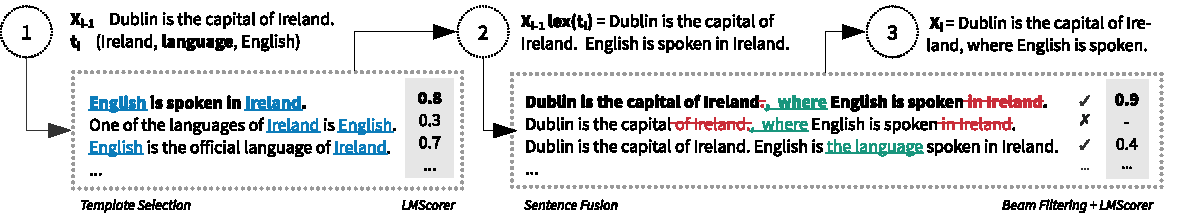
\includegraphics[width=\textwidth]{img/d2t_text_editing}
    \caption[Iterative data-to-text generation.]{A single iteration of our algorithm for iterative \ac{d2t} generation. In Step 1, the template for the triple is selected and filled. In Step 2, the sentence is fused with the template. In Step 3, the result for the next iteration is selected from the beam by filtering and language model scoring.}\label{fig:iterative:alg}
\end{figure*}

\subsection{Implementation}
\label{sec:iterative:implementation}

\begin{table}[t]
    \centering\footnotesize
    \begin{tabular}{@{}lllll@{}}
        \textbf{dataset} & \textbf{method} & \textbf{predicate}          & \textbf{example \#1}                       & \textbf{example \#2}                \\\midrule
        WebNLG           & extracted       & \texttt{foundedBy}          & \et{} was the founder of \eh{}.            & \eh{} was founded by \et{}.         \\
        E2E              & extracted       & \texttt{area}+\texttt{food} & \eh{} offers $\ets$ cuisine in the $\etf$. & \eh{} in $\etf$ serves $\ets$ food. \\
        E2E              & manual          & \texttt{near}               & \eh{} is located near \et{}.               & \et{} is close to \eh{}.
    \end{tabular}
    \caption[Examples of templates used for our experiments.]{Examples of templates we used in our experiments. The markers \eh{} and \et{} are placeholders for the subject and the object, respectively (E2E templates contain two objects). The templates for the single predicates in the WebNLG dataset and the pairs of predicates in the E2E dataset are extracted automatically from the training data; the templates for the single predicates in E2E are created manually.}
    \label{tab:iterative:templates_ex}
\end{table}


We experiment with the WebNLG and E2E datasets. We base our sentence fusion model on the text-editing model \textsc{LaserTagger} \cite{malmi2019lasertagger}, which is a \ac{plm} based on BERT \cite{devlinBERTPretrainingDeep2019}.  As the \textsc{LMScorer} backend, we use the pre-trained GPT-2 language model \citep{radford2019language} from the Huggingface Transformers \citep{wolf2019HuggingFacesTS}. We compute the perplexity scores using the \textit{lm-scorer}\footnote{\url{https://github.com/simonepri/lm-scorer}} package.


\subsection{Experiments}
\label{sec:iterative:experiments}
For the \emph{baseline}, we concatenate the best templates according to \textsc{LMScorer} without applying the sentence fusion (i.e., always using the fallback). For the \emph{sentence fusion} experiments, we use \textsc{LaserTagger} with the autoregressive decoder with a beam of size 10.  Additionally, we conduct a \textit{zero-shot} experiment. We train the sentence fusion model with the same setup, but instead of the in-domain datasets, we use a subset of the \emph{balanced-Wikipedia} portion of the \textsc{DiscoFuse} dataset \cite{geva-etal-2019-discofuse}.


\subsection{Results}
\label{sec:iterative:results}

\begin{table*}[t]
    \centering\footnotesize
    \begin{tabular}{lcccc<{\hspace{1mm}}c>{\hspace{1mm}}cccc} \toprule
                           & \multicolumn{4}{c}{\bf WebNLG} &        & \multicolumn{4}{c}{\bf E2E}                                                                                                                                                  \\
        \cmidrule{2-5} \cmidrule{7-10}
                           & {BLEU}                         & {NIST} & \hspace{-1mm}{METEOR}\hspace{-1mm} & \hspace{-1mm}{ROUGE$_L$}\hspace{-1mm} &  & {BLEU} & {NIST} & \hspace{-1mm}{METEOR}\hspace{-1mm} & \hspace{-1mm}{ROUGE$_L$}\hspace{-1mm} \\
        {\bf baseline}     & 0.277                          & 6.328  & 0.379                              & 0.524                                 &  & 0.207  & 3.679  & 0.334                              & 0.401                                 \\
        {\bf sent. fusion} & 0.353                          & 7.923  & 0.386                              & 0.555                                 &  & 0.252  & 4.460  & 0.338                              & 0.436                                 \\
        {\bf zero-shot }   & 0.288                          & 6.677  & 0.385                              & 0.530                                 &  & 0.220  & 3.941  & 0.340                              & 0.408                                 \\
        {\bf SFC }         & 0.524                          & -      & 0.424                              & 0.660                                 &  & 0.436  & -      & 0.390                              & 0.575                                 \\
        {\bf T5 }          & 0.571                          & -      & 0.440                              & -                                     &  & -      & -      & -                                  & -                                     \\ \bottomrule
    \end{tabular}
    \caption[Results of automatic metrics on WebNLG and E2E]{Results of automatic metrics on the WebNLG and E2E test sets.}
    \label{tab:iterative:results}
\end{table*}
On lexical similarity metrics (\autoref{tab:iterative:results}), our system lags behind the state-of-the-art approaches selected for comparison: the Semantic Fidelity Classifier (SFC; \citealp{harkousHaveYourText2020}) and the finetuned T5 model (T5; \citealp{kaleTexttoTextPreTrainingDatatoText2020}). However, both the fusion and the zero-shot approaches show improvements over the baseline. It is also important to note that our approach ensures zero entity errors by definition: we fill the entities verbatim into the templates, and if an entity is missing in the whole beam, we use a fallback instead (although semantic inconsistencies can still occur, e.g., if a verb or function words are missing).

The zero-shot model trained on \textsc{DiscoFuse} is able to correctly pronominalize or delete repeated entities and join the sentences with conjunctions, e.g.\ \textit{William Anders was born in British Hong Kong\underline{, and was} a member of the crew of Apollo 8}. While the model makes only limited use of sentence fusion, it makes the output more fluent while keeping strong guarantees of the output accuracy.


Our system generates outputs that are suboptimal in fluency when compared with larger models. However, certain unique features make our approach still attractive. Firstly, the approach guarantees the presence of the entities in the output, which is not guaranteed by any approach relying on a \ac{lm} in the final step. Our approach also helps with direct control over the generative process. For example, one can accept or reject the changes at each step or build a set of custom rules for individual edit operations on specific tokens. This possibility can be useful for fine-grained hallucination control \cite{rebuffel2021controlling,chen2023converge} and increasing the robustness of the model in a production system \cite{heidari2021getting,wang2023interactive}.




\section{Pipeline of Text-to-Text Neural Modules}

In this section, we propose using autoregressive \acp{plm} and adding modules for ordering and aggregation, turning the generation process into a three-step pipeline (\Cref{sec:pipeline:method,sec:pipeline:implementation}). We also propose a way to make each of these steps trainable on a generic synthetic corpus (\autoref{sec:pipeline:wikifluent}). We confirm that on WebNLG and E2E datasets, our approach can get lower rates of omissions and hallucinations than prior approaches according to a semantic accuracy metric while achieving levels of lexical similarity comparable to some of the prior systems; all of this without the need for in-domain training data (\Cref{sec:pipeline:experiments,sec:pipeline:eval}).


\subsection{Method}
\label{sec:pipeline:method}
\begin{figure}[t]
    \centering
    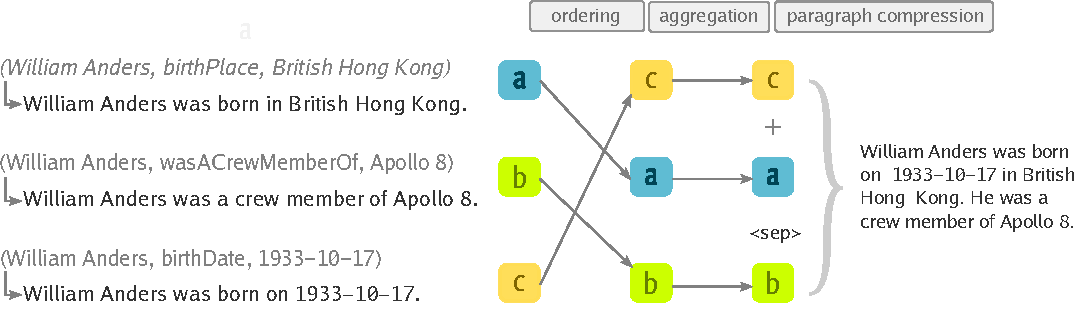
\includegraphics[width=\textwidth]{img/zeroshot_pipeline.pdf}
    \caption[Zero-shot data-to-text generation.]{A scheme of our approach for zero-shot data-to-text generation from RDF triples. After a simple transformation of triples to facts, we apply the pipeline of modules for (1) ordering, (2) aggregation, and (3) paragraph compression. Individual modules are trained on a large general-domain text corpus and operate over text in natural language.}\label{fig:zeroshot:pipeline}
\end{figure}


Similarly to \Cref{sec:finetuning,sec:iterative}, we focus on the task of producing a natural language description $Y$ a set of \ac{rdf} triples $x \in X$, where each triple $x = (s, p, o)$ describes the relation $p$ between the entities $s$ and $o$ in the knowledge graph.

The first step in our pipeline involves transforming each of the input triples $x \in X$ into a fact $f \in F$  using a transformation $T: X \rightarrow F$. We define a fact $f$ as a single sentence in natural language describing $x$.

The second step is the sentence ordering module $O(F)$, which produces an ordered sequence of facts: $F_o = \{f_{o_1}, \ldots, f_{o_n}\}$, where $o_{1:n}$ is a permutation of fact indices. An example outcome of such operation may be ordering adjacently facts mentioning \textit{birth date} and \textit{birth place} of a person, followed by their \textit{occupation}, as it is shown in \autoref{fig:zeroshot:pipeline}. The ordering module allows downstream modules to focus only on operations over neighboring facts.

The third step is the aggregation module, that takes a sequence of ordered facts $F_o$ as input and produces a sequence of sentence delimiters $A(F_o) = \{\delta_{o_1}, \delta_{o_2}, \ldots, \delta_{o_{n-1}}\}$; $\delta_{i} \in \{0, 1\}$. Lastly, the \ac{pc} module takes as input the ordered sequence of facts with delimiters $F_a = \{f_{o_1}, \delta_{o_1}, f_{o_2}, \ldots, \delta_{o_{n-1}}, f_{o_n}\}$ and produces the final text $Y$.


\subsection{\textsc{WikiFluent} Corpus}
\label{sec:pipeline:wikifluent}
We propose a way to build a large-scale synthetic corpus (\textsc{WikiFluent}) for training our modules from English Wikipedia.

For building the \textsc{WikiFluent} corpus, we first extracted 934k first paragraphs of articles from a Wikipedia dump\footnote{\texttt{enwiki-20210401-pages-articles-multistream}} using WikiExtractor \cite{Wikiextractor2015}. We used the first paragraphs of Wikipedia entries with lengths between 30-430 characters, filtering out lists, disambiguations, and malformed paragraphs. To balance the lengths of inputs, we divided the paragraphs according to their length into four equally-sized bins (30-130 characters, etc.) and selected 250k examples from each bin.

\begin{table*}[t]
    \centering
    \footnotesize
    \begin{tabular}{l rrrrrrrr}\toprule
                                              & \bf  \#train & \bf \#dev & \bf \#test & \bf tok/src & \bf tok/tgt & \bf sent/src & \bf sent/tgt \\  \midrule
        WebNLG                                & 18,102       & 870       & 1,862      & 26.8        & 22.6        & 3.0          & 1.4          \\
        Clean E2E                             & 33,236       & 4,299     & 1,847      & 29.2        & 22.3        & 4.2          & 1.5          \\ \midrule
        \textsc{WikiFluent}-\textit{full}     & 915,855      & 9,346     & 9,346      & 52.9        & 41.1        & 3.9          & 2.0          \\
        \textsc{WikiFluent}-\textit{filtered} & 700,517      & 7,149     & 7,149      & 45.6        & 35.4        & 3.4          & 1.8          \\ \bottomrule
    \end{tabular}
    \caption[Statistics of \textsc{WikiFluent} and data-to-text datasets.]{Number of examples (train / dev / test), the average number of tokens per source and target, the average number of sentences per source and target (after filling the templates for the D2T datasets), the total number of templates.}
    \label{tab:pipeline:wikifluent}
\end{table*}

We train BART-base \cite{lewisBARTDenoisingSequencetoSequence2019} for \citep{narayan-etal-2017-split} on the WikiSplit corpus, containing human-made sentence splits from Wikipedia edit history \cite{botha-etal-2018-learning}.  We split each paragraph into sentences using NLTK \cite{bird2006nltk} and apply the split-and-rephrase model to each sentence. We also apply a coreference resolution model \cite{Lee2018HigherorderCR} from the AllenNLP framework \cite{gardner2018allennlp} and we replace referring expressions with their antecedents (e.g., pronouns with noun phrases).

To ensure that the generated sentences convey the same semantics as the original paragraph, we use the RoBERTa model\footnote{\url{https://huggingface.co/roberta-large-mnli}} \cite{liuRoBERTaRobustlyOptimized2019} finetuned on the MultiNLI dataset \cite{williams2018mnli} for filtering the dataset.

\subsection{Implementation}
\label{sec:pipeline:implementation}

We transform triples into facts using a single-triple template $t_i$ for each predicate, analogically to our approach in \autoref{sec:iterative:implementation}, i.e., using the templates extracted from the training data. Compared to more complex rule-based template generation engines \cite{laha2020scalable,heidari2021getting,mehta2021improving}, the approach minimizes manual workload and makes it easier to control the quality of the input for the subsequent steps.

For our ordering model, we use the \emph{Simple Pointer} model from \citet{calizzano2021ordering}. The model is based on a pretrained BART-base model \cite{lewisBARTDenoisingSequencetoSequence2019} extended with a pointer network from \citet{wang2019hierarchical}. We train the model using the synthesized simple sentences in the \textsc{WikiFluent} corpus, randomly shuffling the order of the sentences and training the model to restore their original order.

We base our aggregation model on RoBERTa-large \cite{liuRoBERTaRobustlyOptimized2019} with a token classification head. We input the sequence of ordered facts $F_o$ into the model, separating each pair of facts $f_{o_i}$ with a separator token. The token classification layer classifies each separator token into two classes $\{0,1\}$ corresponding to the delimiter $\delta_i$. We create training examples for aggregation using the synthesized sentences in the \textsc{WikiFluent} corpus, in which we set $\delta_i=0$ for the sentences $i,i+1$ which are the result of splitting a single sentence and $\delta_i=1$ otherwise.

For the paragraph compression model, we finetune BART-base \cite{lewisBARTDenoisingSequencetoSequence2019} on the \textsc{WikiFluent} corpus, concatenating the split sentences on the input and training the model to produce the original, human-written complex sentences on the output. We add delimiters between the sentences $i$ and $i+1$ where $\delta_i=1$ using a special token \texttt{<sep>}, which we add to the model vocabulary.


\subsection{Experiments}
\label{sec:pipeline:experiments}
We train our pipeline modules on the \textsc{WikiFluent} corpus as described in \autoref{sec:pipeline:implementation}. Next, we use these modules \textit{without any further finetuning} for generating descriptions for RDF triples on the WebNLG and E2E datasets.


\begin{figure*}[t]
    \centering
    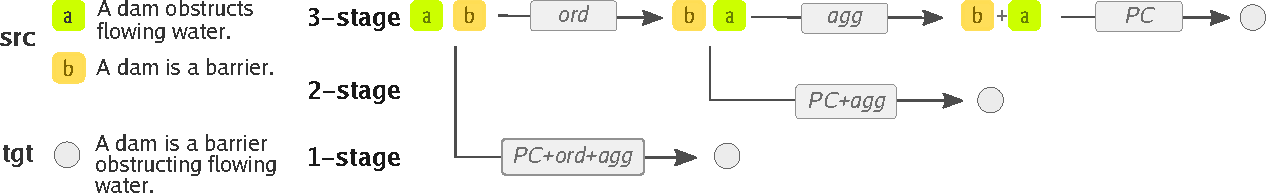
\includegraphics[width=\textwidth]{img/pipeline-variants.pdf}

    \caption[Pipeline variants.]{An example illustrating how the individual modules are trained and subsequently applied as the parts of the pipeline. See \autoref{sec:pipeline:experiments} for the description of the ordering model (\textsc{ord}), the aggregation model (\textsc{agg}), and the variants of the paragraph compression model (\textsc{PC, PC+agg, PC+ord+agg}).}
    \label{fig:pipeline:variants}
\end{figure*}

To evaluate individual components of our pipeline, we train three versions of the \textit{paragraph compression} model (see \autoref{fig:pipeline:variants}): \textsc{\ac{pc}}, \textsc{\ac{pc}+agg}, and \textsc{\ac{pc}+ord+agg}. The models share the same architecture and targets but differ in their inputs. Correspondingly, we test three versions of the pipeline for the ablation study: \textsc{3-stage}, \textsc{2-stage}, and \textsc{1-stage}.

\subsection{Evaluation}
\label{sec:pipeline:eval}
We evaluate outputs from the \textsc{\{1,2,3\}-stage} variants of our pipeline using automatic metrics, and we perform a detailed manual error analysis of the model outputs.


\paragraph{Automatic Metrics}


\begin{table}[t]

    \centering \footnotesize
    \begin{tabular}{llcccccccc} \toprule
                                                                                       &                  & \multicolumn{4}{c}{\textbf{WebNLG}} & \multicolumn{4}{c}{\textbf{E2E}}                                                                                                       \\
                                                                                       &                  & \textbf{B}                          & \textbf{M}                       & \textbf{O}     & \textbf{H}     & \textbf{B}     & \textbf{M}     & \textbf{O}     & \textbf{H}     \\\midrule
        \multicolumn{2}{l}{\baselinecopy{}}                                            & 37.18            & 38.77                               & 0.000                            & 0.000          & 24.19          & 34.89          & 0.000          & 0.000                           \\\cdashlinelr{1-10}
        \multicolumn{2}{l}{$\text{UPF-FORGe}^*$}                                       & 38.65            & 39.00                               & 0.075                            & 0.101          & -              & -              & -              & -                               \\
        \multicolumn{2}{l}{$\textsc{Melbourne}^*$}                                     & 45.13            & 37.00                               & 0.237                            & 0.202          & -              & -              & -              & -                               \\
        \multicolumn{2}{l}{$\text{\citet{keJointGTGraphTextJoint2021}}^{\dagger *}$}   & 66.14            & 47.25                               & -                                & -              & -              & -              & -              & -                               \\
        \multicolumn{2}{l}{$\text{\citet{laha2020scalable}}^{\dagger}$}                & 24.80            & 34.90                               & -                                & -              & -              & -              & -              & -                               \\\cdashlinelr{1-10}
        \multicolumn{2}{l}{\textsc{TGen}$^*$}                                          & -                & -                                   & -                                & -              & 40.73          & 37.76          & 0.016          & 0.083                           \\
        \multicolumn{2}{l}{\citet{harkousHaveYourText2020}$^{\dagger *}$}\hspace{-2mm} & -                & -                                   & -                                & -              & 43.60          & 39.00          & -              & -                               \\\midrule
        \multirow{3}{*}{\textit{full}}                                                 & \textsc{3-stage} & 42.92                               & 39.07                            & 0.051          & 0.148          & \textbf{36.04} & 36.95          & \textbf{0.001} & \textbf{0.001} \\
                                                                                       & \textsc{2-stage} & 42.90                               & 39.28                            & \textbf{0.043} & 0.125          & 35.84          & 36.91          & \textbf{0.001} & \textbf{0.001} \\
                                                                                       & \textsc{1-stage} & 39.08                               & 38.94                            & 0.071          & 0.204          & 30.81          & 36.01          & 0.009          & 0.122          \\\cdashlinelr{1-10}
        \multirow{3}{*}{\textit{filtered}}                                             & \textsc{3-stage} & 43.19                               & 39.13                            & 0.152          & \textbf{0.073} & 35.88          & 36.95          & \textbf{0.001} & \textbf{0.001} \\
                                                                                       & \textsc{2-stage} & \textbf{43.49}                      & \textbf{39.32}                   & 0.146          & 0.096          & 36.01          & \textbf{36.99} & \textbf{0.001} & \textbf{0.001} \\
                                                                                       & \textsc{1-stage} & 42.99                               & 38.81                            & 0.202          & 0.093          & 34.08          & 36.32          & 0.012          & 0.050          \\ \bottomrule
    \end{tabular}
    \caption[Automatic metrics on the WebNLG and E2E datasets]{Automatic metrics on the WebNLG and E2E datasets. B = BLEU, M = METEOR, O = omissions / \# facts, H = hallucinations / \# examples. The systems marked with asterisk (*) are trained on in-domain data. The results for the systems marked with $\dagger$ are taken from the respective works. \textbf{Boldface} denotes the best variant of our zero-shot system.}
    \label{tab:pipeline:auto}
\end{table}

The automatic evaluation (\autoref{tab:pipeline:auto}) shows that our systems consistently outperform the \baselinecopy{} baseline (e.g., $\sim$12 \acs{bleu} points for E2E), which is already strong thanks to our manually curated set of templates.\footnote{On WebNLG, \baselinecopy{} achieves 37.18 \acs{bleu} points, compared to 24.80 \acs{bleu} points of the \textit{full system} of \citet{laha2020scalable}, which uses automatic template generation.} Automatic scores also suggest that our systems are comparable with some older supervised systems, although they underperform the state-of-the-art supervised systems.

The \textsc{2-stage} system is generally on par with the \textsc{3-stage} system, which indicates that explicit aggregation using the \textsc{agg} model may not be necessary. However, a separate aggregation module allows one to control the aggregation step explicitly. The models using the filtered version of the corpus generally produce better results, although they also bring in a larger number of omissions.


% \paragraph{Manual Error Analysis}

% \begin{table}[t]
%     \centering\footnotesize
%     \begin{tabular}{l l ccccc >{\hspace{3mm}}ccccc} \toprule
%          &                  & \multicolumn{5}{c}{\bf WebNLG} & \multicolumn{5}{c}{\bf E2E}                                                                                                         \\
%          &                  & \textbf{H}                     & \textbf{I}                  & \textbf{O} & \textbf{R} & \textbf{G} & \textbf{H} & \textbf{I} & \textbf{O} & \textbf{R} & \textbf{G} \\\midrule
%         \multirow{3}{*}{\textit{full}}
%          & \textsc{3-stage} & 3                              & 39                          & 2          & 2          & 16         & 0          & 1          & 0          & 0          & 17         \\
%          & \textsc{2-stage} & 8                              & 36                          & 1          & 5          & 16         & 1          & 1          & 0          & 1          & 23         \\
%          & \textsc{1-stage} & 28                             & 27                          & 6          & 10         & 20         & 17         & 0          & 1          & 79         & 45         \\\cdashlinelr{1-12}
%         \multirow{3}{*}{\textit{filtered}}
%          & \textsc{3-stage} & 2                              & 37                          & 2          & 1          & 15         & 0          & 0          & 0          & 0          & 17         \\
%          & \textsc{2-stage} & 5                              & 32                          & 1          & 2          & 14         & 0          & 0          & 0          & 0          & 11         \\
%          & \textsc{1-stage} & 8                              & 40                          & 6          & 6          & 16         & 11         & 2          & 1          & 41         & 22         \\\bottomrule
%     \end{tabular}
%     \caption[Number of manually annotated errors on 100 examples]{Number of manually annotated errors on 100 examples: H = hallucinations, I = incorrect fact merging, O = omissions, R = redundancies, G = grammar errors or disfluencies.}
%     \label{tab:pipeline:manual}
% \end{table}


% \begin{table*}[t]\centering\footnotesize
%     \begin{tabular}{l p{12.2cm}} \toprule
%         \textbf{Input}  & \textit{(Allen Forrest; background; solo singer), (Allen Forrest; genre; Pop music), (Allen Forrest; birthPlace; Dothan, Alabama)} \\
%         \textbf{Templ.} & Allen Forrest is a solo singer. Allen Forrest performs Pop music. Allen Forrest was born in Dothan, Alabama.                       \\
%         \textbf{Model}  & \lightblue{Allen Forrest is a solo singer who performs Pop music. He was born in Dothan, Alabama.}                                 \\
%         \textbf{Human}  & Born in Dothan, Alabama, Allen Forrest has a background as a solo singer and was a pop artist.                                     \\\cdashlinelr{1-2}
%         \textbf{Input}  & \textit{name[Wildwood], eatType[restaurant], food[French], area[riverside], near[Raja Indian Cuisine]}                             \\
%         \textbf{Templ.} & Wildwood is a restaurant. Wildwood serves French food. Wildwood is in the riverside. Wildwood is near Raja Indian Cuisine.         \\
%         \textbf{Model}  & \lightblue{Wildwood is a restaurant serving French food. It is in the riverside near Raja Indian Cuisine.}                         \\
%         \textbf{Human}  & A amazing French restaurant is called the Wildwood. The restaurant is near the Raja Indian Cuisine in riverside. They love kids.   \\ \bottomrule
%     \end{tabular}
%     \caption[Example outputs of our model (\textsc{3-stage}, filtered)]{Example outputs of our model (\textsc{3-stage}, filtered). For each example, we show the input triples, the intermediate templates, the output from the model, and the corresponding human reference. Note that in contrast to the model output, the reference contains a typo (``A amazing'') and its style is generally less constrained.}
%     \label{tab:pipeline:ex1}
% \end{table*}

We also manually examined 100 model outputs, counting the number of semantic errors (hallucinations, omissions, incorrect fact merging, redundancies) and grammatical errors. The results are available in the thesis.



% To conclude, our pipeline is inspired by the concept of pipelines based on iterative improvements of simple templates  \cite{laha2020scalable} and neural modules \cite{ferreiraNeuralDatatotextGeneration2019}. We focus on the \emph{ordering} and \emph{aggregation} steps, which were shown to improve the quality of \ac{d2t} generation outputs in domain-specific setups \cite{moryossef2019improving,moryossef2019step,trisedyaSentenceGenerationEntity2020,su2021plan}. In contrast to previous approaches, our pipeline is fully trainable on general-domain data, i.e., without using any training data from target \ac{d2t} datasets. By eliminating the need for human references, we remove the costly and time-consuming data collection process. At the same time, we also avoid the brittleness of few-shot approaches, which are sensitive to the choice of finetuning examples \cite{chenFewShotNLGPreTrained2019,suFewShotTabletoTextGeneration2021,changSelectGenChallengeFinding2021}.


\chapter{Evaluating Semantic Accuracy}
\label{chap:evaluation}
This chapter introduces two metrics for evaluating the semantic accuracy of \ac{d2t} generation. The metrics are predominantly based on \acp{plm} and generic text-to-text operations, which makes our approaches applicable to various tasks and domains.


\section{Detecting Omissions and Hallucinations}
\label{sec:sem-acc}

In this section, we propose a new metric for evaluating the semantic accuracy of \ac{d2t} generation. Our metric is based on a neural model pretrained for \ac{nli}.
We use the \ac{nli} model to check textual entailment between the input data and the output text in both directions, allowing us to reveal omissions or hallucinations (\Cref{sec:sem-acc:method,sec:sem-acc:experiments}).
We demonstrate that even without any extra model training and with minimal handcrafting, our approach achieves high accuracy (>90\%) on the E2E dataset and produces useful results (>75\% accuracy) on the more challenging WebNLG dataset. Additionally, we show with manual error analysis that some instances marked as faults of our metric were in fact assessed correctly by our metric (\autoref{sec:sem-acc:evaluation}).

\subsection{Method}
\label{sec:sem-acc:method}
We are given a set of \acs{rdf}\glsunset{rdf} triples $x \in X$, where each triple $x = (s, p, o)$ describes the relation $p$ between the entities $s$ and $o$, and the corresponding natural language description $Y$. Our task is to assess whether $Y$ mentions all the triples in $X$. Additionally, we should also check whether the text mentions any extra information.

We used simple templates for transforming individual triples to facts, i.e., simple sentences capturing the triple meaning, similarly to \autoref{chap:low-res}.

% \paragraph{Natural Language Inference} \ac{nli} is a sequence classification task that takes two inputs---a \textit{hypothesis} and a \textit{premise}---and produces one of the possible outputs: the hypothesis is \textit{entailed} by (follows from) the premise, \textit{contradicts} the premise, or their relation is \textit{neutral}. Neural models for \ac{nli} \cite{zhang2019semantics,liu-etal-2019-multi,liuRoBERTaRobustlyOptimized2019} have already reached near-human levels of performance, making them suitable for evaluating the output of abstractive summarization systems \cite{maynezFaithfulnessFactualityAbstractive2020}.


\paragraph{Checking Semantic Accuracy with NLI} We use an \ac{nli} model for assessing the semantic accuracy of generated texts. Consider the two input facts from \autoref{fig:sem-acc:ex}: $F= $\{\emph{``Blue spice is a pub''}, \emph{``Blue Spice is located in the riverside''}\} and the generated text: $Y= $\emph{``You can bring your kids to Blue Spice in the riverside area.''} We propose using an \ac{nli} model for checking if the semantic information implied by $F$ and $Y$ is equal.
In this case, the model should detect an omission, i.e., that the first fact is not entailed by the text (there is no mention of Blue Spice being a pub), and also a hallucination, i.e., that the text is not entailed by the facts (the information about kids is superfluous).

We achieve this by using the \ac{nli} model to check for entailment in two directions:
\begin{enumerate}
    \item To check for \textrm{omissions}, we use the whole generated text as a premise and sequentially feed each fact as a hypothesis to the \ac{nli} model. Any failed \ac{nli} check is considered an omission.
    \item To check for \textrm{hallucinations}, we concatenate all facts as a premise and feed the generated text as a hypothesis to the \ac{nli} model. If this \ac{nli} check fails, the text is considered to contain hallucination. This step cannot be split into simpler \ac{nli} checks.
\end{enumerate}


\begin{figure*}[t]
    \centering
    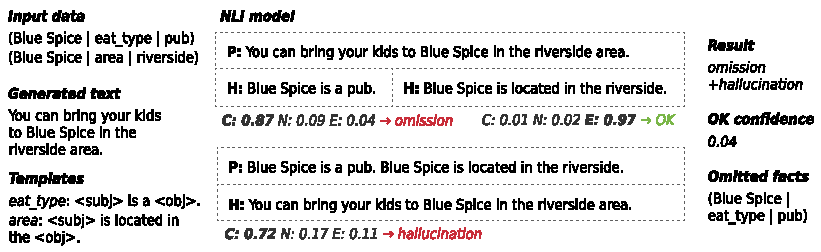
\includegraphics[width=\textwidth]{img/2020_nli_inlg}
    \caption[Our semantic accuracy metric.]{An example of evaluating the output from a \ac{d2t} system with our metric. The generated text is used as a \textit{premise} (\textit{P}) to check for omissions and as a \textit{hypothesis} (\textit{H}) to check for hallucinations. The \ac{nli} model generates probabilities for \textit{contradiction} (\textit{C}), \textit{neutral} (\textit{N}) and \textit{entailment} (\textit{E}).}
    \label{fig:sem-acc:ex}
\end{figure*}

The final output of our metric is either 4-way (denoted as \textsc{Fine}) or 2-way (denoted as \textsc{Rough}):
\begin{itemize}
    \item \textsc{Fine}: We output the probabilities of 4 categories: \emph{OK} (i.e., all \ac{nli} checks passed), \emph{omission}, \emph{hallucination}, or \emph{omission+hallucination} (based on the failed checks). The 4-way output is more useful for system evaluation since we can distinguish whether the system tends to hallucinate or omit information.
    \item  \textsc{Rough}: The three failure modes are combined into \emph{not\_OK}. The 2-way output corresponds more to usage inside an \ac{d2t} generation system for output reranking or filtering, where any incorrect output should be penalized or filtered out.
\end{itemize}

Additionally, we compute a \textit{confidence score} of the model as the minimum of all the entailment probabilities.


\subsection{Experiments}
\label{sec:sem-acc:experiments}
For our \ac{nli} model, we use the \texttt{roberta-large-mnli}\footnote{\scalebox{0.95}[1.0]{\url{https://huggingface.co/roberta-large-mnli}}} checkpoint of the pretrained RoBERTa model \cite{liuRoBERTaRobustlyOptimized2019}, which was finetuned on the Multi\ac{nli} dataset \cite{williams2018mnli}. We use the model \textit{as is}, without any further training on domain-specific data.
Given a premise text and a hypothesis text, the \ac{nli} model produces a probability distribution over three results: \textit{contradiction}, \textit{neutral},
and \textit{entailment} (see \autoref{sec:sem-acc:method}). We consider a \ac{nli} check as passed if the probability for \textit{entailment} is the highest of the three.


We experiment with the WebNLG and E2E datasets, similarly as in \autoref{chap:low-res} (see \autoref{sec:datasets} for the descriptions of the datasets). Since both datasets were used in shared tasks, we can compare the outputs of our system with the respective measures of semantic accuracy:
\begin{itemize}
    \item For WebNLG, we compare our metric with crowdsourced human ratings of semantic adequacy \cite{shimorinaWebNLGChallengeHuman2019}. In particular, we use the answers for the question: \textit{``Does the text correctly represent the meaning in the data?''}, where the human annotators used a three-point Likert scale (1 = Incorrect, 2 = Medium, 3 = Correct). The answers are averaged over multiple annotators. In our experiments, we consider a sentence correct if it achieved a human rating of 2.5 or higher.\footnote{We also tried a threshold of 2.0, with slightly worse results.}
    \item For E2E, we compare our metric to the results of the handcrafted automatic script which was used in the E2E challenge \cite{dusekEvaluatingStateoftheartEndtoEnd2020}.\footnote{While the E2E challenge did include crowdsourced evaluation of semantic accuracy, the results were unreliable, overestimating the number of errors \cite{dusekEvaluatingStateoftheartEndtoEnd2020}.}

\end{itemize}

We experiment with the \emph{Default} and \emph{Backoff} approaches to transforming triples to facts, as described in \autoref{sec:sem-acc:method}. For WebNLG, we obtained templates by delexicalizing human references for single-triple examples from the WebNLG training data. For E2E, we handcrafted eight templates for each predicate in the dataset.\footnote{For each predicate in WebNLG, we choose randomly if more templates are found and use the backoff if no templates are found. Note that for E2E, we did \emph{not} use the complex templates extracted from the training data (cf. \autoref{chap:low-res}).}



\begin{table}[t]
    \centering \small
    \begin{tabular}{l ccccc>{\hspace{3mm}}ccccc} \toprule
                & \multicolumn{5}{c}{\bfseries WebNLG} & \multicolumn{5}{c}{\bfseries E2E}                                                                                                                  \\
                & \textbf{A}                           & \textbf{R}                        & \textbf{P} & \textbf{F1} & $\mathbf{\rho}$ & \textbf{Af} & \textbf{Ar} & \textbf{R} & \textbf{P} & \textbf{F1} \\\midrule
        Default & 0.775                                & 0.772                             & 0.796      & 0.784       & 0.628           & 0.911       & 0.933       & 0.895      & 0.910      & 0.903       \\
        Backoff & 0.768                                & 0.760                             & 0.793      & 0.776       & 0.637           & 0.846       & 0.874       & 0.913      & 0.768      & 0.834       \\ \bottomrule
    \end{tabular}
    \caption[Results of our metric on WebNLG and E2E.]{WebNLG and E2E results, compared to crowdsourced human ratings and the automatic evaluation script, respectively (A = accuracy, Af = \textsc{Fine} accuracy, Ar = \textsc{Rough} accuracy, R = recall, P = precision, F1 = F-measure, $\rho$ = Spearman correlation of confidence scores with human scores).}
    \label{tab:sem-acc:res}
\end{table}

\subsection{Evaluation}
\label{sec:sem-acc:evaluation}

We evaluate our metric in terms of accuracy (\textbf{A}), precision (\textbf{P}), recall (\textbf{R}), and F1-measure\footnote{We treat \emph{not\_OK} samples as positive since we focus on detecting errors.} (\textbf{F1}) with respect to the corresponding ground truth outputs. For WebNLG, we additionally compute Spearman correlation coefficient ($\rho$) of the model's confidence scores with the average human scores. For E2E, we evaluate the accuracy for both the \textsc{Fine} (\textbf{Af}) and \textsc{Rough} (\textbf{Ar}) variants described in \autoref{sec:sem-acc:method}, making use of the fact that the automatic script reports both omissions and hallucinations. The scores for both datasets are summarized in \autoref{tab:sem-acc:res}.

We additionally perform a manual error analysis on a random sample of 100 error examples for each dataset, i.e., examples where our metric gave a different assessment from the ground truth.


\paragraph{WebNLG Analysis}  The overall scores (between 77-80\% for all measures) show that our metric deviates quite a lot from human judgments. Our manual error analysis indicates several potential sources of discrepancies:
\begin{enumerate}
    \item The human annotation is somewhat noisy---many correctly rendered outputs do not reach the 2.5 threshold, while some incorrect ones do.
    \item The human annotators also tend to give lower scores to accurate but ungrammatical or poorly organized texts, while our metric tends to rate these texts as \emph{OK}.
    \item Imprecise templates can confuse the \ac{nli} (e.g., for the predicate \emph{nationality}, our extracted template is \emph{\textless{}subj\textgreater{} was \textless{}obj\textgreater{}}, which works well with values such as \emph{French}, but not with \emph{United States}). This is a weak point of our metric, as illustrated by the very small performance difference between the \emph{Default} and \emph{Backoff} setups. However, the issue can be mitigated by a better selection of the templates from training data, e.g., using language-model scoring.
\end{enumerate}

The Spearman correlation of our model's confidence scores with the average human scores is around 0.63 ($p<$1e-10). This is similar to n-gram-based metrics on this data (\citet{shimorina2018human} reports 0.59 for BLEU and 0.73 for METEOR), but unlike these metrics, our approach does not require human-written reference texts.

Moreover, our re-examination shows that almost half of the error examples (42 out of 100) were in fact correctly classified by our metric (i.e., their crowdsourced human annotation was incorrect),  so the true performance is most likely higher than the reported numbers.


\paragraph{E2E Analysis} The results for the E2E dataset are very good compared to the WebNLG dataset, with over 90\% agreement with the handcrafted script. This can be attributed to lower lexical variability and less noisy texts, as well as to the better quality of the handcrafted templates (the difference between the \emph{Default} and \emph{Backoff} setups is much more pronounced here). The main issues identified by our error analysis are:
\begin{enumerate}
    \item Problems in the interpretation of some values, e.g., \textit{price range=less than \textsterling{}20} is verbalized as ``cheap'' or \textit{family-friendly=no} as ``adult-only''. These cases are classified as \emph{not\_OK} by the \ac{nli} model.
    \item Missing or over-greedy patterns in the slot error script, causing annotation errors.
    \item Edge cases: some expressions cannot be interpreted in a straightforward way, e.g., ``high restaurant'' for \emph{pricerange=high} is deemed OK by the \ac{nli} but not by the slot error script.
    \item Expressions in the outputs that do not correspond to input facts, such as ``with full service'', are considered hallucinations by the \ac{nli} but ignored by the slot error script.
\end{enumerate}
Again, we consider about half of the error examples (45 out of 100) as correctly classified by our metric, and thus our metric's performance is probably higher than the reported values.


\subsection{Discussion}

\paragraph{Comparison to Other Metrics} Automatic metrics for assessing semantic accuracy of text are mostly reference-based \cite{zhaoMoverScoreTextGeneration2019,dhingraHandlingDivergentReference2019,sellam2020bleurt,ronyRoMeRobustMetric2022} or targetting tasks with non-structured inputs such as summarization, paraphrasing, or fact verification \cite{honovich2022true,zha2023alignscore}, which makes their use-cases different from ours. The closest alternative to our metric is Data-QuestEval \cite{rebuffel2021data}: a metric based on a question generation and question answering model, which is trained on a synthetic dataset containing structured data on the input.
In the future, a more flexible metric for evaluating semantic accuracy could be based on large language models \cite{zhaoInvestigatingTabletoTextGeneration2023,sottanaEvaluationMetricsEra2023,kocmiLargeLanguageModels2023}, a topic to which we return in \autoref{sec:quintd}.

\paragraph{Limitations} Perhaps surprisingly, the main bottleneck of the metric is not in the capabilities in \ac{nli} model. Although the \ac{nli} model is not perfect, \citet{chenMENLIRobustEvaluation2022} have shown that out-of-the-box \ac{nli} models are generally better and more robust metrics than specially trained approaches. In many cases, however, converting the structured data to a format suitable to \ac{plm} can be non-trivial. In this respect, we would like to refer to the discussion on automating template generation with \acp{plm} and \acp{llm} in \autoref{sec:pipeline:discussion}.


\section{Token-Level Error Classification}
\label{sec:tok-eval}

\begin{refbox}
    This section is based on the paper \emph{Text-in-Context: Token-Level Error Detection for Table-to-Text Generation} \cite{kasnerTextinContextTokenLevelError2021}, joint work with Simon Mille and Ondřej Dušek, published in the Proceedings of the 14th International Conference on Natural Language Generation (INLG 2021). The work describes our submission to the Shared Task on Evaluating Accuracy in Generated Texts. The project was led by the author of the thesis, Simon Mille provided the rule-based generator and wrote its description, Ondřej Dušek supervised the project.
\end{refbox}


In this section, we present an automatic metric for fine-grained detection of semantic accuracy errors in \ac{d2t} generation outputs. In contrast with the example-level metric introduced in  \autoref{sec:sem-acc}, the metric we introduce here can detect the hallucination errors on the level of individual \emph{tokens}.\footnote{For the purpose of this section, the term \emph{token} denotes the output of word-level tokenization as implemented in NLTK \cite{bird2006nltk}, mostly consisting of individual words or punctuations signs.} The metric combines a rule-based \ac{d2t} generation system and \acp{plm} (\autoref{sec:tok-eval:system}). We first use a rule-based \ac{d2t} generation system to generate all facts that can be derived from the input as short natural-language
sentences (cf. \autoref{sec:sem-acc}). For each sentence we evaluate, we select a subset of relevant facts by measuring their semantic similarity with the examined sentence. For annotating erroneous tokens, we finetune a pretrained language model for token-level classification, using the annotated data with the relevant facts in the context as the ground truth.

On the test set of the Shared Task on Evaluating Accuracy in Generated Texts \cite{thomsonGenerationChallengesResults2021}, we achieve 69\% recall and 75\% precision with a model trained on a mixture of human-annotated and synthetic data, placing first out of four submissions in the track for automatic metrics (\autoref{sec:tok-eval:experiments}). The code for our experiments is available on Github.\footnote{\url{https://github.com/kasnerz/accuracySharedTask_CUNI-UPF}}


\subsection{Motivation}
\label{sec:tok-acc:motivation}


In \autoref{sec:sem-acc}, we presented a metric for detecting semantic errors in \ac{d2t} generation at the level of individual data items. The metric is well-suited for cases where the text should mention \emph{all the data on the input}, as it can report individual missing items (omissions). However, it is less suitable for detecting incorrect information in the text (hallucinations), as it can give only a single ``hallucination score'' for the entire text. This is problematic for the texts generated from complex data, where the omissions are not relevant (since we do not verbalize all the input data), but the system can still produce numerous hallucinations.


An example of a dataset with complex data is Rotowire (\citealp{wiseman2017challenges}; see \autoref{sec:datasets} for details). In this dataset, the task is to generate basketball match summaries from tabular data. Rotowire poses multiple challenges for neural systems, including the fact that it requires content selection or that its human-written training texts are themselves not always grounded in data, which makes neural models more susceptible to hallucination \cite{dusekSemanticNoiseMatters2019}.
The output texts are also usually longer, which makes the hallucinations more common and detecting hallucination errors on a more fine-grained level essential.

There is, however, no established way to check for hallucinations automatically. Specific content-checking metrics mostly remain a domain of handcrafted pattern matching \cite{wen2015semantically,dusekSemanticNoiseMatters2019}, which does not scale well to new domains. While human evaluation provides a more reliable alternative, it is costly and difficult to set up \cite{van2019best,belzDisentanglingPropertiesHuman2020,thomsonGoldStandardMethodology2020}. Neural metrics such RoMe \cite{ronyRoMeRobustMetric2022} or Data-QuestEval \cite{rebuffel2021data} do not target specifically content preservation, especially not on the level of individual tokens.


\subsection{Shared Task in Evaluating Accuracy}
\label{sec:tok-acc:st}
The goal of the Shared Task on Evaluating Accuracy in Generated Texts at INLG 2021 was to develop a token-level error annotation metric for complex \ac{d2t} generation \cite{reiterSharedTaskEvaluating2020}. The organizers of the shared task first manually annotated 60 outputs of various neural systems trained on Rotowire, using the error types defined in \citet{thomsonGoldStandardMethodology2020}:
\begin{itemize}
    \item \errnum{NUMBER} --  Incorrect number (both digits and numerals).
    \item \errent{NAME} -- Incorrect named entity (people, places, teams, days of the week).
    \item \errword{WORD} -- Incorrect word which is not one of the above.
    \item \errctx{CONTEXT} --  A phrase inappropriate for the context.
    \item \errnc{NOT\_CHECKABLE} --  A statement which cannot be checked.
    \item \errother{OTHER} --  Any other type of mistake.
\end{itemize}
\begin{figure}[t]
    \footnotesize
    \lineacross{}


    The Memphis Grizzlies (5-\errnum{2}) defeated the Phoenix Suns (3 - 2) \errent{Monday} 102-91 at the \errent{Talking Stick Resort Arena} in Phoenix. The Grizzlies had a \errword{strong} first half where they \errword{out-scored} the Suns \errnum{59}-\errnum{42}. Marc Gasol scored 18 points, \errword{leading} the Grizzlies.  \errctx{Isaiah Thomas added} 15 points, he is \errnc{averaging 19 points on the season so far}.
    \vspace{1mm}

    \begin{itemize}
        \item \errnum{2}                                       -- Incorrect number, should be 0.
        \item \errent{Monday}                                  -- Incorrect named entity, should be Wednesday.
        \item \errent{Talking Stick Resort Arena}              -- Incorrect named entity, should be US Airways Center.
        \item \errword{strong}                                 -- Incorrect word, the Grizzlies did not do well in the first half.
        \item \errword{out-scored}                             -- Incorrect word, the Suns had a higher score in first half.
        \item \errnum{59}                                      -- Incorrect number, should be 46.
        \item \errnum{42}                                      -- Incorrect number, should be 52 .
        \item \errword{leading}                                -- Incorrect word.  Marc Gasol did not lead the Grizzlies, Mike Conley did with 24 points.
        \item \errctx{Isaiah Thomas added}                     -- Context error.  Thomas played for the Suns, but context here implies he played for the Grizzlies and added to their score.
        \item \errnc{averaging 10 points on the season so far} -- Not checkable.  This is very hard to check, since data sources report performance per season and per game, not performance up to a particular point in a season.
    \end{itemize}
    \lineacross{}

    \caption[An example text with error annotations.]{Example text with error annotations adapted from \citet{thomsonGenerationChallengesResults2021}, using the error marking style from \citet{thomsonEvaluatingFactualAccuracy2023}. The original data for this game is available at \url{https://www.basketball-reference.com/boxscores/201411050PHO.html} .}
    \label{fig:tok-eval:example}
\end{figure}
An example of an annotated system output is provided in \autoref{fig:tok-eval:example}. The objective of the shared task was to either implement an automatic metric for creating the same type of annotations automatically or to develop a human evaluation scenario capable of producing the same annotations while requiring fewer resources.



\subsection{Our System}
\label{sec:tok-eval:system}

\begin{figure*}[t]
    \centering
    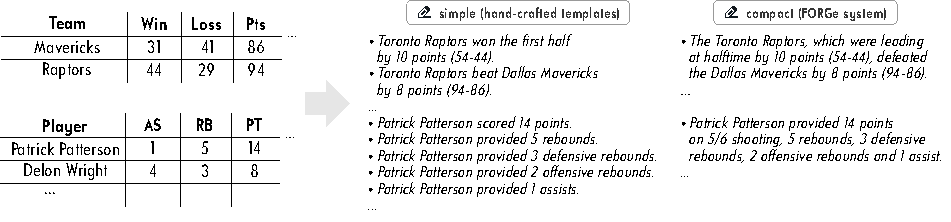
\includegraphics[width=\textwidth]{img/tok-eval_generator.pdf}
    \caption[Our rule-based systems for generating facts from the input data.]{Rule-based system that we use to generate facts from the input data. The facts are used as input to the error-checking model (see \autoref{fig:tok-eval:system}). We experiment with (a) simple hand-crafted templates and (b) compact sentences generated by the FORGe system.}
    \label{fig:tok-eval:gen}
\end{figure*}





Our submission for the shared task falls into the first category: we developed an automatic metric based on a \ac{plm}, that marks each token in the output text for the presence of errors. To make the tabular input data understandable for the \ac{plm}, we use a rule-based system to exhaustively generate all the facts that can be derived from the data.\footnote{Similarly to \Cref{sec:pipeline,sec:sem-acc}, we represent the fact as short sentences.} Since the context window of the \ac{plm} underlying the metric is limited, we also use a neural-based retrieval system to retrieve only $c$ relevant facts, which are added into the context window of the \ac{plm} to support its decisions. We describe the individual components of our system below.



\paragraph{Rule-based Fact Descriptions}
We use a rule-based system to generate facts from the input tables in natural language. For each game, we generate facts about the game (hosting team, visiting team, date converted to weekday), line-score objects (team name and statistics), and box-score objects (player name, player team, player starting position and their personal statistics). We also generate additional facts that can be inferred from the input table, such as which team won and by how much, comparisons between the team and player raw data (e.g., \emph{Team A and Team B committed the same number of fouls}), details based on statistics (e.g., \emph{Player X recorded a double-double}), or an interpretation of some numbers (e.g., \emph{Team A came back in the 4th quarter}).\footnote{A number of facts frequently mentioned in human-written descriptions could not be obtained from the Rotowire data, as for instance the player stats per quarter, a career-high points total, whether a player is an all-star or not, or if a player scored the winning shot. These facts thus cannot be checked with our system.}

We experiment with both \emph{simple} descriptions created by filling in sentence templates and \emph{compact} descriptions generated using a grammar-based system:
\begin{itemize}
    \item \textbf{Simple descriptions} are produced by a template-based system, with one template per fact. We handcrafted 129 sentence templates to cover all the facts described above. A sentence template looks like the following: ``\textit{[PLAYER$\_$NAME] scored [PTS] points.}'', where square brackets indicate variables that are instantiated with the corresponding input values (see Figure~\ref{fig:tok-eval:gen} for sample sentences).
    \item  \textbf{Compact descriptions} are produced by the FORGe system \cite{mille2019teaching}, that allows for the generation of more compact sentences.  For instance, the five bottom sentences from the simple system in \autoref{fig:tok-eval:gen} are covered by the single bottom sentence from the compact system. FORGe performs surface realization in several steps, by first aggregating the templates based on the predicate and argument identity and then structuring, linearizing, and inflecting components of the sentences. The FORGe grammars were used off-the-shelf,\footnote{We deactivated cross-sentence referring expression generation so that each generated sentence can be used independently.} with additional 98 manually crafted abstract templates.
\end{itemize}

The simple system produces about 569 facts for each game. The compact system covers the same amount of information with more syntactically complex sentences, producing about 112 sentences per game, i.e., five times less.


\begin{figure*}[t]
    \centering
    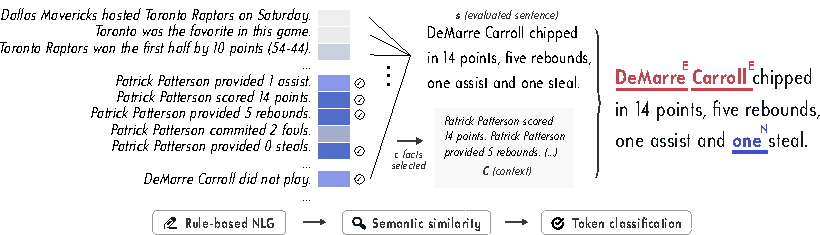
\includegraphics[width=\textwidth]{img/tok-eval_system.pdf}
    \caption[Our system for token-level error annotation.]{An overview of our system. First, we generate the facts from the input table with a rule-based NLG system (see \autoref{fig:tok-eval:system}). For each evaluated sentence $s$, we select $c$ facts with the highest semantic similarity, getting a context $C$. The pair $(C, s)$ is given as an input to a pretrained LM for token-level error classification.}
    \label{fig:tok-eval:system}
\end{figure*}

\paragraph{Context Retrieval} The maximum length of the input sequence for our error tagger (see \autoref{sec:tok-eval:experiments}) is 512 tokens, which is about 10\% of the total length of the generated sentences $G$. Therefore, we select only a subset of $G$, which we refer to as \emph{context} $C$. For each generated sentence $g_i\in G$, we measure semantic similarity between $g_i$ and the evaluated sentence $s$ using Sentence Transformers \cite{reimers-gurevych-2019-sentence}. In particular, we embed the sentence tokens by applying mean pooling on the output of \texttt{paraphrase-distilroberta-base-v2}, getting the embedding vectors $e_{s}$ and $e_{g_i}$. Then, we compute the cosine similarity between the embeddings:
\begin{align}
    score = \frac{e_s \cdot e_{g_i}}{\lVert e_s \rVert \lVert e_{g_i} \rVert}.
\end{align}
For the context $C$, we select the top $c$ sentences from $G$ that have the highest cosine similarity to $s$.


\paragraph{LM-based Error Tagger}
As our error tagger, we use RoBERTa \cite{liuRoBERTaRobustlyOptimized2019} with a token-level classification head. The model receives an input $X = (C, s)$ and is trained to annotate each token in $s$ either with an \textit{OK} label or with a label corresponding to one of the error categories. We experiment with two data sources for training the model:
\begin{itemize}
    \item \emph{gold-standard annotated data} from the shared task (which contains all error types),
    \item \emph{synthetic data} created by perturbing the human-written summaries from Rotowire (which contains only \errent{NAME} and \errnum{NUMBER} errors).
\end{itemize}

\paragraph{Synthetic Data} The gold-standard data contains only 60 games, as opposed to 3,395 games in the Rotowire training set. This led us to the idea of using the training set as a source of synthetic data, introducing errors into human-written descriptions. We focus only on the \errent{NAME} and \errnum{NUMBER} errors, i.e., the categories that are the most represented and also easiest to generate. In each sentence, we identify named entities in the text using \emph{spaCy}.\footnote{\url{https://spacy.io}} We modify only a certain portion of entities according to the \emph{entity modification rate} (EMR), which we treat as a hyperparameter. We introduce the \errent{NAME} errors by:
\begin{enumerate}
    \item swapping the names of teams with opponent teams,
    \item swapping the names of players with other players in the game,
    \item swapping the names of cities with other cities in the Rotowire dataset,
    \item swapping the days of the week.
\end{enumerate}
For \errnum{NUMBER} errors, we take an integer $n$ identified in the text, sample a number from a normal distribution with $\mu=n$ and $\sigma=3$, and truncate it to get an integer. We re-sample if the output equals the original number or for negative outputs. If the number is spelled out, we use \texttt{text2num}\footnote{\url{https://pypi.org/project/text2num/}} and  \texttt{num2words}\footnote{\url{https://pypi.org/project/num2words/}} to convert to digits and back.


\subsection{Experiments}
\label{sec:tok-eval:experiments}

For the error tagger, we train a PyTorch version of RoBERTa from the Huggingface Transfomers repository \cite{wolf2019HuggingFacesTS} using the AdamW optimizer \cite{loshchilov2018fixing}, learning rate $5\times10^{-5}$ and linear warmup.
We finetune the model for 10 epochs and select the model with the highest validation score.
We experiment with several hyperparameters:
\begin{itemize}
    \item \emph{simple} vs.~\emph{compact} sentences in $G$,
    \item  \textit{number of sentences} retrieved for the context: $c$ = 5, 10, 20 or 40;
    \item \textit{entity modification rate} (EMR): proportion of entities modified in the synthetic data: 0.25, 0.5, or 0.75.
\end{itemize}
We evaluate the model using a script provided by the organizers, which computes recall and precision of the model output with respect to the human-annotated data. Since we use the human-annotated data for training, we perform 6-fold cross-validation: in each run, we use 45 games for training, 5 games for validation, and 10 games for evaluation.


\begin{table*}[!htbp]
    \centering\footnotesize
    \begin{tabular}{@{}l l r >{\hspace{2mm}} ccc >{\hspace{2mm}} ccc >{\hspace{2mm}} ccc@{}}\toprule
        \multirow{2}{*}{\bf Gen.}                    & \multirow{2}{*}{\bf Data} & \multirow{2}{*}{$c$} & \multicolumn{3}{c}{\bf EMR = 0.25} & \multicolumn{3}{c}{\bf EMR = 0.5} & \multicolumn{3}{c}{\bf EMR = 0.75}                                                         \\
                                                     &                           &                      & R                                  & P                                 & F1                                 & R         & P     & F1    & R         & P     & F1    \\\midrule
        \multirow{8}{*}{\bf\rotatebox{90}{Simple} }  & \multirow{4}{*}{s}
                                                     & 5                         & 0.123                & 0.723                              & 0.210                             & 0.165                              & 0.512     & 0.250 & 0.310 & 0.323     & 0.316         \\
                                                     &                           & 10                   & 0.138                              & 0.737                             & 0.232                              & 0.181     & 0.549 & 0.272 & 0.328     & 0.400 & 0.360 \\
                                                     &                           & 20                   & 0.137                              & \bf 0.741                         & 0.231                              & 0.179     & 0.559 & 0.271 & 0.327     & 0.433 & 0.373 \\
                                                     &                           & 40                   & 0.165                              & 0.712                             & 0.268                              & 0.199     & 0.560 & 0.294 & 0.296     & 0.436 & 0.353 \\\cdashlinelr{2-12}
                                                     & \multirow{4}{*}{s+h}
                                                     & 5                         & 0.422                & 0.617                              & 0.501                             & 0.414                              & 0.594     & 0.488 & 0.401 & 0.583     & 0.475         \\
                                                     &                           & 10                   & 0.467                              & 0.551                             & 0.506                              & 0.438     & 0.638 & 0.519 & 0.428     & 0.665 & 0.521 \\
                                                     &                           & 20                   & 0.518                              & 0.640                             & 0.573                              & 0.544     & 0.575 & 0.559 & 0.509     & 0.595 & 0.549 \\
                                                     &                           & 40                   & 0.584                              & 0.644                             & \bf 0.613                          & \bf 0.595 & 0.612 & 0.603 & 0.519     & 0.639 & 0.573 \\\midrule
        \multirow{8}{*}{\bf \rotatebox{90}{Compact}} & \multirow{4}{*}{s}
                                                     & 5                         & 0.151                & \bf 0.696                          & 0.248                             & 0.170                              & 0.617     & 0.267 & 0.336 & 0.427     & 0.376         \\
                                                     &                           & 10                   & 0.176                              & 0.663                             & 0.278                              & 0.195     & 0.624 & 0.297 & 0.295     & 0.486 & 0.367 \\
                                                     &                           & 20                   & 0.196                              & 0.672                             & 0.303                              & 0.205     & 0.635 & 0.310 & 0.278     & 0.552 & 0.370 \\
                                                     &                           & 40                   & 0.166                              & 0.643                             & 0.264                              & 0.197     & 0.595 & 0.296 & 0.306     & 0.530 & 0.388 \\ \cdashlinelr{2-12}
                                                     & \multirow{4}{*}{s+h}
                                                     & 5                         & 0.600                & 0.641                              & 0.620                             & 0.552                              & 0.635     & 0.591 & 0.588 & 0.600     & 0.594         \\
                                                     &                           & 10                   & 0.583                              & 0.662                             & 0.620                              & 0.629     & 0.606 & 0.617 & \bf 0.656 & 0.606 & 0.630 \\
                                                     &                           & 20                   & 0.622                              & 0.647                             & 0.634                              & 0.597     & 0.688 & 0.639 & 0.600     & 0.660 & 0.629 \\
                                                     &                           & 40                   & \cellcolor{hlyellow}0.614          & \cellcolor{hlyellow}0.690         & \bf \cellcolor{hlyellow}0.650      & 0.609     & 0.630 & 0.619 & 0.611     & 0.630 & 0.620 \\\bottomrule
    \end{tabular}
    \caption[Results of our system on development data.]{Recall (R), precision (P) and F1 scores on development data. $s$ stands for synthetic training data and $h$ for human training data.  $c$ indicates the number of sentences in the context provided to the tagger, EMR stands for entity modification rate. Best recall, precision and F1 scores for both generators (simple and compact) are shown in bold, the submitted model is highlighted in yellow.}
    \label{tab:tok-eval:results}
\end{table*}

\paragraph{Development Results} The results of our model on the development data are listed in Table \ref{tab:tok-eval:results}. For our final submission, we selected the model with the best F1-score overall, which is 0.65 (0.61 recall and 0.69 precision). The model uses 40 compact sentences in context, 0.25 EMR, and was trained on both synthetic and human-annotated data. Although compact texts are generally helpful, there are also some well-performing models using simple templates only. A higher number of sentences in context may help to achieve a better F1-score, but not always (the longer context is also sometimes cropped to fit the input). Using a higher EMR then generally leads to higher recall, suggesting that the model adapts to the base rate of errors.

\begin{table}[t]
    \centering\small
    \begin{tabular}{l cccc}\toprule
        \multirow{2}{*}{\bf Error Type} & \multicolumn{2}{c}{\bf Mistake} & \multicolumn{2}{c}{\bf Token}                 \\
                                        & R                               & P                             & R     & P     \\ \midrule
        \errent{NAME}                   & 0.750                           & 0.846                         & 0.759 & 0.862 \\
        \errnum{NUMBER}                 & 0.777                           & 0.750                         & 0.759 & 0.752 \\
        \errword{WORD}                  & 0.514                           & 0.483                         & 0.465 & 0.529 \\
        \errctx{CONTEXT}                & 0.000                           & -                             & 0.000 & -     \\
        \errnc{NOT\_CHECKABLE}          & 0.000                           & -                             & 0.000 & -     \\
        \errother{OTHER}                & 0.000                           & -                             & 0.000 & -     \\ \noalign{\vskip 0.1cm}\hdashline\noalign{\vskip 0.1cm}
        \textbf{Overall}                & 0.691                           & 0.756                         & 0.550 & 0.769 \\\bottomrule
    \end{tabular}
    \caption[Results of our system on test data.]{Results of our system on test data: recall (R) and precision (P) are shown for individual error types.}
    \label{tab:tok-eval:results-test}
\end{table}

\paragraph{Submission Results}
Table \ref{tab:tok-eval:results-test} shows the results of our model on the official test data of the task, broken down by error types. The overall scores are higher than on the development set -- test set recall is 0.69 (vs.~0.61 on the development set), and precision is 0.76 (vs.~0.69). The fact that we used all the available human-annotated data for training the final model may have contributed to the difference, but it is also possible that the test data was somewhat less challenging. We note that our model was able to identify only three types of errors (\errent{NAME}, \errnum{NUMBER}, \errword{WORD}), having better results for the \errent{NAME} and \errnum{NUMBER} errors. We believe the explanation is two-fold: the names and numbers are often found verbatim in the input data (and in our generated facts), which makes them easy to detect, and also the corresponding error types were the most represented in the training data. In contrast, the three error types that were not detected are much less represented in the training data and are hard to detect in our setup.


\subsection{Discussion}
\paragraph{Limitations} Our metric depends on the existence of a rule-based system for generating factual statements from the data. Such a system may be hard to develop, even though we have shown that simple templates can be similarly efficient as more complex approaches. As our approach is data-driven, it also requires system outputs annotated with errors. This requirement may be partially mitigated by using synthetic data. In our case, using synthetic data only results in low recall (see \autoref{tab:tok-eval:results}), but more sophisticated techniques for creating the synthetic data may lead to better results.

\paragraph{How to Improve The Metric} Our submission achieved the best results in the automatic metrics category, but there is still a gap with what humans can achieve, as shown by the Laval University submission's overall 0.84 recall and 0.88 precision \cite{garneau2021laval}. One way to improve our system would be to enrich the reference fact descriptions by either inferring more information from the raw data or by extracting additional data from external databases. Another option would be to add surrounding sentences to the context -- this could help to resolve coreferences (e.g. if a player is referred to as \textit{"He"}) and to detect the \errctx{CONTEXT} errors.

\paragraph{LLM-based Alternatives} Recently, the evaluation metrics based on \acp{llm} are starting to provide an alternative, more flexible approach for evaluating generated texts \cite{kocmiGEMBAMQMDetectingTranslation2023,zhaoInvestigatingTabletoTextGeneration2023,sottanaEvaluationMetricsEra2023,chiang-lee-2023-large,fu2023gptscore}. An advantage of the \ac{llm}-based metrics is the possibility of defining custom error categories without the need for having annotated data for finetuning the model. We explore such an approach in \autoref{sec:quintd}, where we use a \ac{llm}-based metric for token-level evaluation of generated text. However, it should be noted that with \ac{llm}-based metrics, greater flexibility is traded for lower controllability (especially in the case of closed models), making the evaluation potentially biased and hard to reproduce \cite{stureborgLargeLanguageModels2024,kooBenchmarkingCognitiveBiases2023,wangLargeLanguageModels2023}.

\section{Conclusion}
We introduced two metrics for evaluating the semantic accuracy of \ac{d2t} generation. The metric presented in \autoref{sec:sem-acc} targets the cases where all the data items need to be mentioned in the output text. It uses a combination of simple templates and an off-the-shelf neural model, making our approach applicable with minimal additional effort. The metric introduced in \autoref{sec:tok-eval} then targets complex data-to-text generation, using a combination of a rule-based system, a neural retriever, and a neural token-level classifier. While this metric requires in-domain training data, it enables annotating semantic errors on the level of individual tokens. Future research directions may include removing the need for rule-based preprocessing and improving the flexibility with respect to the output error categories.
%
% TEXT END
%
% \renewcommand*{\acronymname}{List of Abbreviations}
% \printglossary[type=\acronymtype,style=index]


% \renewcommand{\chapterheadstartvskip}{\vspace*{0mm}} % chapter spacing

% \cleardoublepage{}
\bibliographystyle{csplainnat}
{\small \bibliography{references}}

% \cleardoublepage{}
\chapter*{List of Publications}

\phantom{\nobibliography*{references}}

% -----------------------------------------------------------------------------

\noindent\bibentry{kasnerTrainHardFinetune2020}
\begin{itemize}[noitemsep,topsep=0pt]

    \item The data-to-text generation system based on the finetuned mBART model (\autoref{sec:finetuning}).
    \item Our submission for the WebNLG+ shared task.
    \item Citations (without self-citations): 9
\end{itemize}\vspace{.5\baselineskip}

% -----------------------------------------------------------------------------
\noindent\bibentry{kasnerDatatoTextGenerationIterative2020}
\begin{itemize}[noitemsep,topsep=0pt]
    \item The data-to-text generation system based on iterative text editing (\autoref{sec:iterative}).
    \item Citations (without self-citations): 17

\end{itemize}\vspace{.5\baselineskip}

% -----------------------------------------------------------------------------
\noindent\bibentry{kasner2022neural}
\begin{itemize}[noitemsep,topsep=0pt]
    \item The data-to-text generation system based on a pipeline of neural modules (\autoref{sec:pipeline}).
    \item Citations (without self-citations): 21

\end{itemize}\vspace{.5\baselineskip}

% -----------------------------------------------------------------------------
\noindent\bibentry{dusekEvaluatingSemanticAccuracy2020}
\begin{itemize}[noitemsep,topsep=0pt]

    \item The metric for detecting omissions and hallucinations in generated texts (\autoref{sec:tok-eval}).
    \item Best short paper at INLG 2020.
    \item Citations (without self-citations): 47

\end{itemize}\vspace{.5\baselineskip}


% -----------------------------------------------------------------------------
\noindent\bibentry{kasnerTextinContextTokenLevelError2021}
\begin{itemize}[noitemsep,topsep=0pt]
    \item The metric for token-level error detection in generated texts (\autoref{sec:tok-eval})
    \item Our submission to the shared task Evaluating Accuracy in Generated Texts.
    \item Citations (without self-citations): 6

\end{itemize}\vspace{.5\baselineskip}


% -----------------------------------------------------------------------------
\noindent\bibentry{kasnerTabGenieToolkitTabletoText2023}
\begin{itemize}[noitemsep,topsep=0pt]

    \item The toolkit for processing and visualization of data-to-text generation datasets (\autoref{sec:tabgenie}).
    \item Citations (without self-citations): 2

\end{itemize}\vspace{.5\baselineskip}


% -----------------------------------------------------------------------------
\noindent\bibentry{kasnerMindLabelsDescribing2022}
\begin{itemize}[noitemsep,topsep=0pt]

    \item The analysis of verbalizing relations in knowledge graphs with pretrained language models (\autoref{sec:rel2text}).
    \item Citations (without self-citations): 3

\end{itemize}\vspace{.5\baselineskip}


% -----------------------------------------------------------------------------
\noindent\bibentry{kasnerReferenceBasedMetricsAnalyzing2024}
\begin{itemize}[noitemsep,topsep=0pt]

    \item The analysis of data-to-text generation with open large language models (\autoref{sec:quintd}).
    \item Citations (without self-citations): 2

\end{itemize}\vspace{.5\baselineskip}

\vfill

\noindent Only publications relevant to this thesis are included. The number of
citations was computed using Semantic Scholar API. Total number of citations of
publications related to the topic of the thesis (without self-citations) by June 14, 2024: {\bf 107}.


\end{document}
